% LaTeX-Vorlage zur Erstellung von Abschlussarbeiten an der FH Aachen
% Author: Sven Hinz
% Aenderung für FB 5: Ingo Elsen

\documentclass[12pt,a4paper]{book}
% Paket für Umlaute:
\usepackage[utf8]{inputenc}       % Cross Platform
%\usepackage[ansinew]{inputenc}   % Windows
%\usepackage[latin1]{inputenc}    % Linux
%\usepackage[applemac]{inputenc}  % Mac

%\usepackage[ngerman]{babel}       % Sprache: deutsch
\usepackage[utf8]{inputenc} % For degree symbol in tex source
\usepackage{amsmath}
\usepackage{amsfonts}
\usepackage{amssymb}
\usepackage{makeidx}
\usepackage{graphicx}
\usepackage{epstopdf}
%\usepackage{kpfonts}
\usepackage{textcomp}
\usepackage[left=2cm,right=2cm,top=2.5cm,bottom=2.5cm]{geometry}
%\usepackage[plainheadsepline,headsepline]{scrpage2}
\usepackage{color}
\usepackage{setspace}
%\usepackage[numbers,square]{natbib} % only required for unsrtd bib style
\usepackage{longtable}
\usepackage{listings}
\usepackage{rotating}
\usepackage{pdfpages}
\usepackage{caption}
\usepackage{subcaption}
\usepackage{float}
\parindent 0pt
\usepackage{booktabs}
\usepackage[export]{adjustbox}
\usepackage{titlesec}
\usepackage{mathtools}

\titleformat{\chapter}[display]
{\normalfont\bfseries}{}{0pt}{\Large}

\newcommand{\TODO}[1]{\textbf{\textcolor{red}{$<$TODO: #1$>$}}}
\newcommand{\NOTE}[1]{\textcolor{cyan}{NOTE: #1}}

\DeclarePairedDelimiter\Floor\lfloor\rfloor
\DeclarePairedDelimiter\Ceil\lceil\rceil


% Schriftart
%\usepackage{courier}
%\usepackage{helvet}
%\usepackage{times}
%\renewcommand{\familydefault}{\sfdefault}
%\renewcommand{\familydefault}{\rmdefault}
%\setkomafont{chapter}{\sffamily \large}
%\setkomafont{section}{\sffamily \normalsize}
%\setkomafont{subsection}{\sffamily \normalsize}
%\setkomafont{subsubsection}{\sffamily \normalsize}
%\addtokomafont{caption}{\sffamily \small}

\setlength{\parindent}{0.5cm}
% Abstand zwischen Kopfzeile und Kapitelüberschrift
%\renewcommand*{\chapterheadstartvskip}{\vspace*{-0.75\baselineskip}}

% Einstellungen der Kopf- und Fußzeile
%\pagestyle{scrheadings}
%\ihead[\sffamily \bfseries \upshape \headmark]{\sffamily \bfseries \upshape %\headmark}
%\chead[]{}
%\ohead[]{}
%\ifoot[]{}
%\cfoot[]{}
%\ofoot[\sffamily \pagemark]{\sffamily \pagemark}
%\automark[]{chapter}
%\renewcommand*{\chapterheadendvskip}{\vspace*{1\baselineskip}}

% Formeln
\usepackage{fleqn} % linksbündig
\setlength{\mathindent}{1.5cm} % Einrücktiefe

% Tabellen
\usepackage{multirow} % mehrzeiliger Text in einer Spalte
\renewcommand{\arraystretch}{2} % Zeilenabstand vergrößern
\setlength{\doublerulesep}{0.1mm} % Abstand der Doppellinien verkleinern
\usepackage{tabu}
\newcolumntype{C}{>{\centering\arraybackslash$}p{3cm}<{$}}

% Quellcode / Kommandozeileneingabe
\lstdefinestyle{BashInputStyle}{
  language=bash,
  basicstyle=\small\ttfamily,
  %numbers=left,
  %numberstyle=\tiny,
  %numbersep=3pt,
  frame=tb,
  columns=fullflexible,
  %backgroundcolor=\color{yellow!20},
  linewidth=0.9\linewidth,
  xleftmargin=0.1\linewidth
}

% Inhalt
%\renewcaptionname{ngerman}{\contentsname}{Inhalt} % Umbenennung in Inhalt

% Quellenverzeichnis
%\renewcaptionname{ngerman}{\bibname}{Quellenverzeichnis} % Umbenennung in Quellenverzeichnis

%\usepackage[
%  tocindentmanual,
%  tocflat,
%  tocbreaksstrict,
%  toctextentriesleft,
%]{tocstyle}

% Abkürzungsverzeichnis
%\usepackage[intoc]{nomencl}
%\let\abbrev\nomenclature
%\renewcommand{\nomname}{Abkürzungsverzeichnis}
%\setlength{\nomlabelwidth}{.25\hsize}
%\renewcommand{\nomlabel}[1]{#1 \dotfill}
%\setlength{\nomitemsep}{-\parsep}
%\makenomenclature

\usepackage[]{acronym}


\author{Vorname Nachname} % --> Eigenen Namen einfügen


\begin{document}
\setstretch{1.1}
\addtocontents{toc}{\linespread{1}}

% Einbinden der Textinhalte mit '\include{...}'
% Die Dateien mit den Textinhalten befinden sich im Ordner 'doc'

\begin{titlepage}
	%ab hier kleinere Raender, mehr bedruckbare Flaeche.
	%\fontfamily{\sffamily}\selectfont
	\thispagestyle{empty}
	\newgeometry{a4paper, portrait, left=0cm, right=0cm, top=0.6cm, bottom=0cm, includefoot}

	% FH Logo
	\begin{flushright}
		
\includegraphics[width=1.7cm]{./pic/FHAC.jpg}
	\end{flushright}

	\vspace{-2.5cm}

	% Kopfzeile mit Fachbereich ...
	\centering \sffamily \bfseries \Large FH~Aachen \\
	\vspace{0.5cm}
	\normalsize Fachbereich\\
	Elektrotechnik und Informationstechnik

	\vspace{1cm}

	\centering \bfseries Bachelorarbeit
	%\centering \bfseries Masterarbeit

	\vspace{0.8cm}

	%Titel der Arbeit
	\centering \begin{minipage}[t]{17cm}
		\centering \bfseries \large Erzeugung eines künstlichen Datensatzes zur Bremsprognose von Güterzügen und Validierung der Big Data Verarbeitung
		\medskip
	\end{minipage}

	\vspace{1.5cm}

	%Name und Matrikelnummer
	%\vspace*{1cm}
	%\hspace*{6.8cm}
	\begin{minipage}[t]{9cm}
		\centering Simon Westfechtel \\ Matr.-Nr.: 3120254
	\end{minipage}

	\vspace{2.1cm}

	%Professor und Betreuer
	%\vspace*{4.7cm}
	%\hspace*{6.8cm}
	\centering \begin{minipage}[t]{9cm}
		\centering \begin{tabular}{ll}
			Referent: & Prof. Dr-Ing. Ingo Elsen\\
			Korreferent: & Prof. Dr. Raphael Pfaff\\
			%Externer Betreuer: & Dipl.-Wirt.-Ing\\
		\end{tabular}
	\end{minipage}

	\vspace{7cm}

	% Firmenlogo
	%\begin{flushleft}
	%\centering \hspace{-8cm}
	%\begin{minipage}[t]{5cm}
			%\includegraphics[width=5cm]{./pic/firmenlogo.jpg}
	%\end{minipage}
	%\end{flushleft}


	%Erstellungsdatum
	%\vspace{-4cm}
	%\begin{flushright}
	\centering %\hspace{8cm}
	\begin{minipage}[b]{5cm}
			\centering
			\today\\ %Datum\\
			%\vspace{1cm}
			%In Zusammenarbeit mit\\
			%Firma, Ort\\
			%\vspace{1cm}
			%vertraulich bis xx.xx.xx
	\end{minipage}
	%\end{flushright}

	%\today
	\restoregeometry
\end{titlepage}


\clearpage
\chapter*{Erklärung}\label{erklaerung}
\markboth{Erklärung}{Erklärung}
Ich versichere hiermit, dass ich die vorliegende Arbeit selbstständig verfasst und keine anderen als die im Literaturverzeichnis angegebenen Quellen benutzt habe.

\bigskip

\noindent
Stellen, die wörtlich oder sinngemäß aus veröffentlichten oder noch nicht veröffentlichten Quellen entnommen sind, sind als solche kenntlich gemacht.

\bigskip

\noindent
Die Zeichnungen oder Abbildungen in dieser Arbeit sind von mir selbst erstellt worden oder mit einem entsprechenden Quellennachweis versehen.

\bigskip

\noindent
Diese Arbeit ist in gleicher oder ähnlicher Form noch bei keiner anderen Prüfungsbehörde eingereicht worden.

\vspace{1cm}
\noindent
Aachen, \today %Monat Jahr

\vspace{7cm}
%\section*{Geheimhaltung}\label{geheimhaltung}

%{\large\textbf{Geheimhaltung}}\\


%Die vorliegende Arbeit unterliegt bis ... der Geheimhaltung. Sie darf vorher weder vollständig noch auszugsweise ohne schriftliche Zustimmung des Autors, des betreuendes Referenten bzw. der Firma ... vervielfältigt, veröffentlicht oder Dritten zugänglich gemacht werden.

\clearpage
\chapter*{Danksagung}\label{danksagung}
\markboth{Danksagung}{Danksagung}
Danke.

% Inhaltsverzeichnis
\clearpage
\makeatletter
\renewcommand*{\@dotsep}{1} % Punktabstand einstellen
\makeatother
\tableofcontents

% Das erste Kapitel soll auf einer ungeraden Seite beginnen.
\cleardoublepage
\setstretch{1.1}

% Nicht benötigte Kapitel können auskommentiert werden
% Für zusätzliche Kapitel müssen weitere Dateien im Ordner 'doc' angelegt werden

%\clearpage
\chapter{\textbf{Einleitung}}\label{einleitung}
%\addtocontents{toc}{\vspace{0.8cm}}


%\par\medskip


\section{Motivation und Aufgabenstellung}
%\addtocontents{toc}{\vspace{0.8cm}}



%% Beispiel für das Einfügen einer Abbildung

%\begin{figure}[h]
%	\centering
%		\includegraphics[width=0.8\textwidth]{pic/dateiname.png}
%	\caption{Beispielbild}
%	\label{fig:beispielbild}
%\end{figure}
%\vspace{7cm} % Abstand unter dem Bild


\newpage

\section{Vorgehensweise}
\addtocontents{toc}{\vspace{0.8cm}} % -> Abstand im Inhaltsverzeichnis

% Untersuchungsverlauf(pro Kapitel ein kurzer Absatz mit Verweis auf die Kapitelnummer)
 % Einleitung
%\clearpage
\chapter{\textbf{Grundlagen}}\label{grundlagen}
%\addtocontents{toc}{\vspace{0.8cm}}

\section{Unterkapitel}\label{unterkapitel}
\addtocontents{toc}{\vspace{0.8cm}}

Wir sehen im Folgenden die Formel für die Faltung von Wahrscheinlichkeitsdichtefunktionen, als Gleichungsarray:

\begin{align}
(p_i * p_j)(n) & =  \sum_{k \in \mathbb{D}} p_i(k) \cdot p_j(n - k) \\
p_{total} & =  p_0 \ast p_1 \ast \ldots p_{n-1}; \forall n
\end{align}

% Formel
Hier ist nur eine einfache Formel mit der \texttt{equation}-Umgebung für die Minkowski Metrik:
\begin{equation}\label{Minkowski}
D\left(X,Y\right)=\left(\sum_{i=1}^n |x_i-y_i|^p\right)^{1/p}\\
\end{equation}

Wie in Gleichung \ref{Minkowski} zu erkennen ist, ergibt sich die L2-Norm (Euklidische Distanz), wenn man den Exponenten $p = 2$ wählt.

Support Vector Machines \cite{Haykin99} nutzen die Euklidische Distanz (oder äquivalent) das Skalarprodukt.
%% Zwei Abbildungen, die zusammen gehören

%\begin{figure}
%        \centering
%        \begin{minipage}[c]{0.45\textwidth}
%                \includegraphics[height=6.5cm]{pic/dateiname1.png}
%        \end{minipage}
%        \begin{minipage}[c]{0.45\textwidth}
%                \includegraphics[height=6.5cm]{pic/dateiname2.png}
%        \end{minipage}
%        \caption{Zwei Abbildungen}\label{fig:zwei_abb}
%\end{figure}

%\clearpage
\chapter{\textbf{Kapitel 3}}\label{kap3}
\addtocontents{toc}{\vspace{0.8cm}}

\begin{table}[htb]
\caption{Messergebnisse}
\label{tab:messung}
\centering
\begin{tabu}{l|[2pt]C|C|C}
Stellung & \frac{T_U}{^\circ C}  & \frac{T_c}{^\circ C} & \frac{\Delta T}{^\circ C}  \\
\tabucline[2pt]{-}
senkrecht (0°) & 27,3 & 69,8 & 42,5\\
\tabucline[0.5pt]{-}
waagerecht (90°) & 26,6 & 70,6 & 44,0\\
\end{tabu}
\end{table}

\begin{table}[h]
\centering
\caption{Smartphone Sensordaten}
\begin{tabu}{|p{9cm}|l|l|}
\hline
Sensorinformation&Format&frequency [$s^{-1}$]\\
\hline
App identifier for vendor & int64 & once per transfer\\
WIFI and network carrier IP addresses& int128 & once per transfer\\
battery level& int8 & 0.1\\
Position information: latitude, longitude, altitude, speed, course, vertical position accuracy, horizontal position accuracy, floor level information& float32[8] & 1\\
Heading information: heading.x, heading.y, heading.z, true heading, magnetic heading, heading accuracy& float16[6] & 1 \\
Accelerometer information: acceleration.x, acceleration.y, acceleration.z& float16[3] & 2 \\
Gyroscope information: rotationRate.x, rotationRate.y, rotationRate.z& float16[3] & 2 \\
altimeter information: relative altitude, pressure & float16[2] & 1 \\ 
timestamp & uint32 & once per transfer \\
Temperature [°C] & float16 & 1\\
\hline
\end{tabu}
\label{tab:smartphonesensor}
\end{table}

Wie in Tabelle \ref{tab:smartphonesensor} zu sehen ist, ist es besser, Trennlinien nur dort einzusetzen, wo logische Grenzen liegen.
%\clearpage
\chapter{\textbf{Zusammenfassung und Ausblick}}\label{zusammenfassung}
\addtocontents{toc}{\vspace{0.8cm}}

\clearpage
%\section{Abstract}
%\label{sec:Abstract}

\par\noindent
\textit{\textbf{Abstract}} Modern day railway system operations require automated train control mechanisms, e.g. European Train Control System ETCS, to maximize efficiency, which is often times limited by outdated infrastructure, as well as safety of operations. One way to achieve this is by lowering the required distance between two trains on the same track, which in turn demands a reliable method of predicting the braking distance at any given moment. 
\par
While determination of the necessary braking curves is feasible for a limited number of train formations, the large diversity of vehicles in freight operations poses an issue. One approach for a solution would be using Big Data, which would be able to process the required amounts of data to calculate reliable braking curves even for freight operations. 
\par
The problem here is there is simply not enough data available since freight trains usually don't have the sensory equipment needed. To circumvent that obstacle, this work proposes generation of artificial data via white box modeling to be then used in further big data operations.
\chapter{Introduction}
\label{chap:Introduction}
\par\noindent
\textit{\textbf{Introduction}} This section describes the background and motivation of the research (section \ref{sec:Background}), the problem to be addressed (section \ref{sec:Problem}) and the proposed solution (section \ref{sec:Solution}).

\section{Background}
\label{sec:Background}
\par\noindent
In recent years, data science has become more and more prominent. Since large quantities of data have become omnipresent, big data processing is applicable in various fields of research and operations. This work focuses on the application of big data processing to railway system operations, more specifically the preconditions. Mainly, two areas show promise to benefit from big data usage, which is predictive maintenance as well as optimization of railway operations. As the name suggests, lots of data is required, think hundreds of terabyte for freight operations in Germany alone. As it stands though, unfortunately, this data source remains largely untapped today, owing to freight wagons typically lacking necessary sensory equipment. This is where this work comes into play.

\subsection{Railway Vehicle Operations}
\label{sec:RailwayVehicleOperations}
\par\noindent
Road and rail traffic are fundamentally different, mainly in two regards. First, the physical properties, which will be discussed in chapter \ref{chap:FundamentalsOfRailwayVehicleEngineering}, second, the actual modalities of operations, which will be topic of this section.
\par
In road traffic, there are many different vehicles, all operating independently from one another. Although there is ongoing experimentation to utilize autonomous vehicles to recreate train-like lorry configurations, this is not the norm. In contrast to that, the track guiding of wheels offered by rails enables the formation of trains possibly kilometers long, reducing labor cost, infrastructure usage and energy consumption. This, of course, calls for special safety measures to be taken, since higher speeds and payloads result in long braking distances. 

\begin{figure}[H]
	\centering
	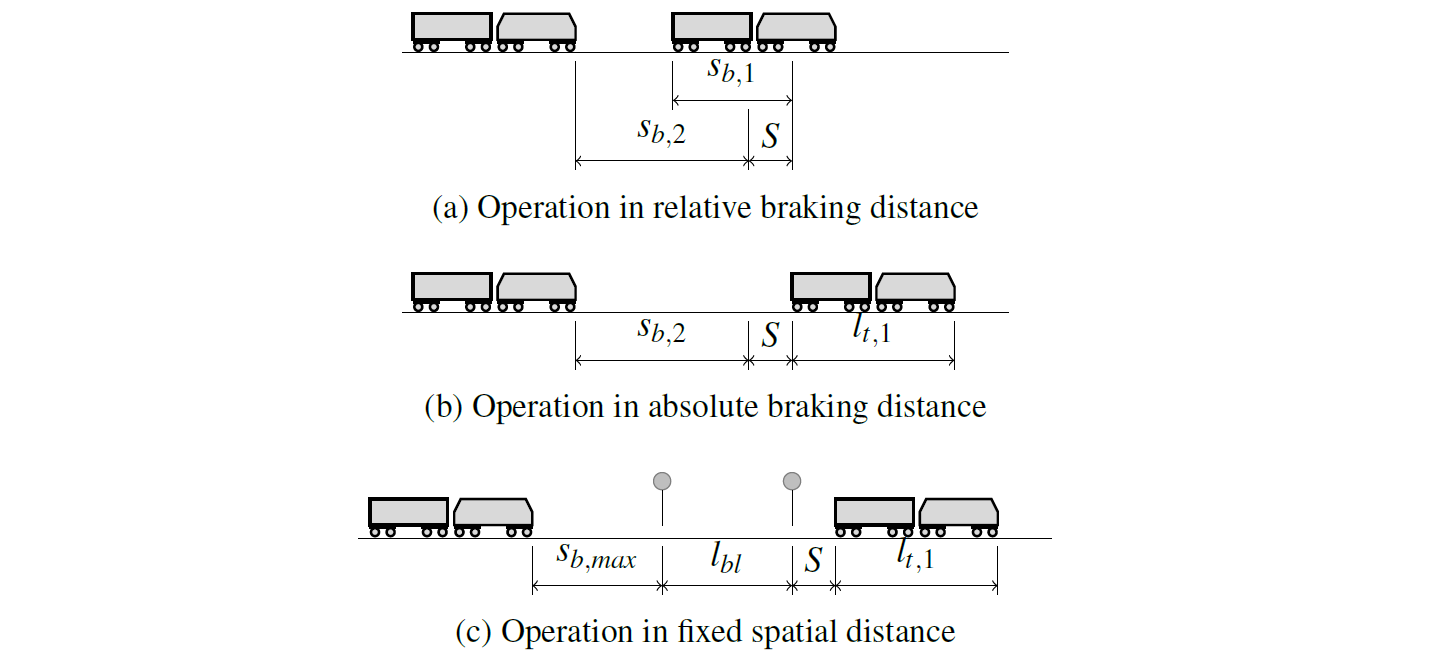
\includegraphics[width=\linewidth]{./pic/abstaende}
	\caption{Spacing paradigms \cite{Pfaff2017}}
	\label{fig:train_spacing}
\end{figure}

\par\noindent
Figure \ref{fig:train_spacing} illustrates the three main principles of spacing between two trains on the same track. $s_{b,i}$ denotes the braking distance of train $i$, $l_{t,i}$ the length of train $i$, $l_{bl}$ the length of a track section, and $S$ a safety margin. In fixed spatial distance, the distance between two trains must at least be the maximum braking distance $S_{b,max}$, plus the length of one track section (i.e. between two signals) $l_{bl}$, plus a safety margin $S$. In absolute braking distance, the distance between two trains must at least be the braking distance of the second train $S_{b,2}$, plus a safety margin $S$. Finally, in relative braking distance, the distance between two trains must be sufficient for the second train to be able to come to a full halt behind the first train if both trains start breaking at the same time. Fixed spatial distance, the most commonly used today, is very inefficient in terms of track utilization, but offers the most protection against accidents. In order to optimize efficiency, it is desirable to move towards relative braking distances, which requires the ability to very accurately predict braking capacity of trains.

\subsection{Automatic Train Protection and Cab Signaling}
\label{sec:ATPCS}
\par\noindent
Automatic train protection systems are designed to ensure safe operation in case of human or technical error or malpractice by the train operator. Generally, all trains operate on track sections which are free of other vehicles, reserved and locked. Think for example a section between two signals. These sections are also referred to as movement authority, and a train has to be capable of coming to a complete halt before the end of movement authority as to not violate a track section locked by another train. For this, the driver and/or the onboard computer needs to be informed about the endpoint of the current movement authority as well as speed limits. The train protection system enforces application of brakes in case of violation of restrictions, for example if the train exceeds the speed limit or the train would otherwise be unable to stop in time before movement authority expires. Train protection systems may be categorized by means of information transfer. Spatially discrete acting systems use transmitters placed at strategic points along the track, for example signals, whereas continuous systems may transmit information at all times, either via track-sided wire loops or radio communication. These allow higher degrees of automation than discrete systems, as trains have access to the necessary real-time data.
\par
Cab signaling relays all relevant information to the train operators so they may act in the most optimal way. The European train control system, short ETCS, encompasses both of these (\cite{Havryliuk2017}, p.12).

\subsection{Braking Curves}
\label{sec:BrakingCurves}
\par\noindent
For the ETCS to be able to supervise train velocity, it needs to determine the vehicle's braking capacity for any given moment in time, using a mathematical model of the braking dynamics and of the track characteristics. This prediction is called a braking curve, which describes the probable braking process for a set of input parameters. For an example, refer to figure \ref{fig:brakingcurves}. It shows a braking process, in particular the decline of the train's velocity over distance. Since braking performance cannot be predicted with absolute certainty, an $\epsilon$ parameter needs to be factored in to account for random behavior. Therefore, there is a number of discrete braking curves for any set of parameters, forming a probability distribution \cite{Pfaff2017}. The parameters may be classified in four categories:
\begin{itemize}
	\item Physical parameters, which are determined by real time measurements from on-board equipment
	\item Fixed values, like driver reaction time
	\item Trackside data, like track gradient or signaling data
	\item Train data, mostly captured beforehand, relating to the rolling stock braking system itself
\end{itemize}
The fourth category, train data, is the key factor for this work, as will be explained below.

\begin{figure}[H]
	\centering
	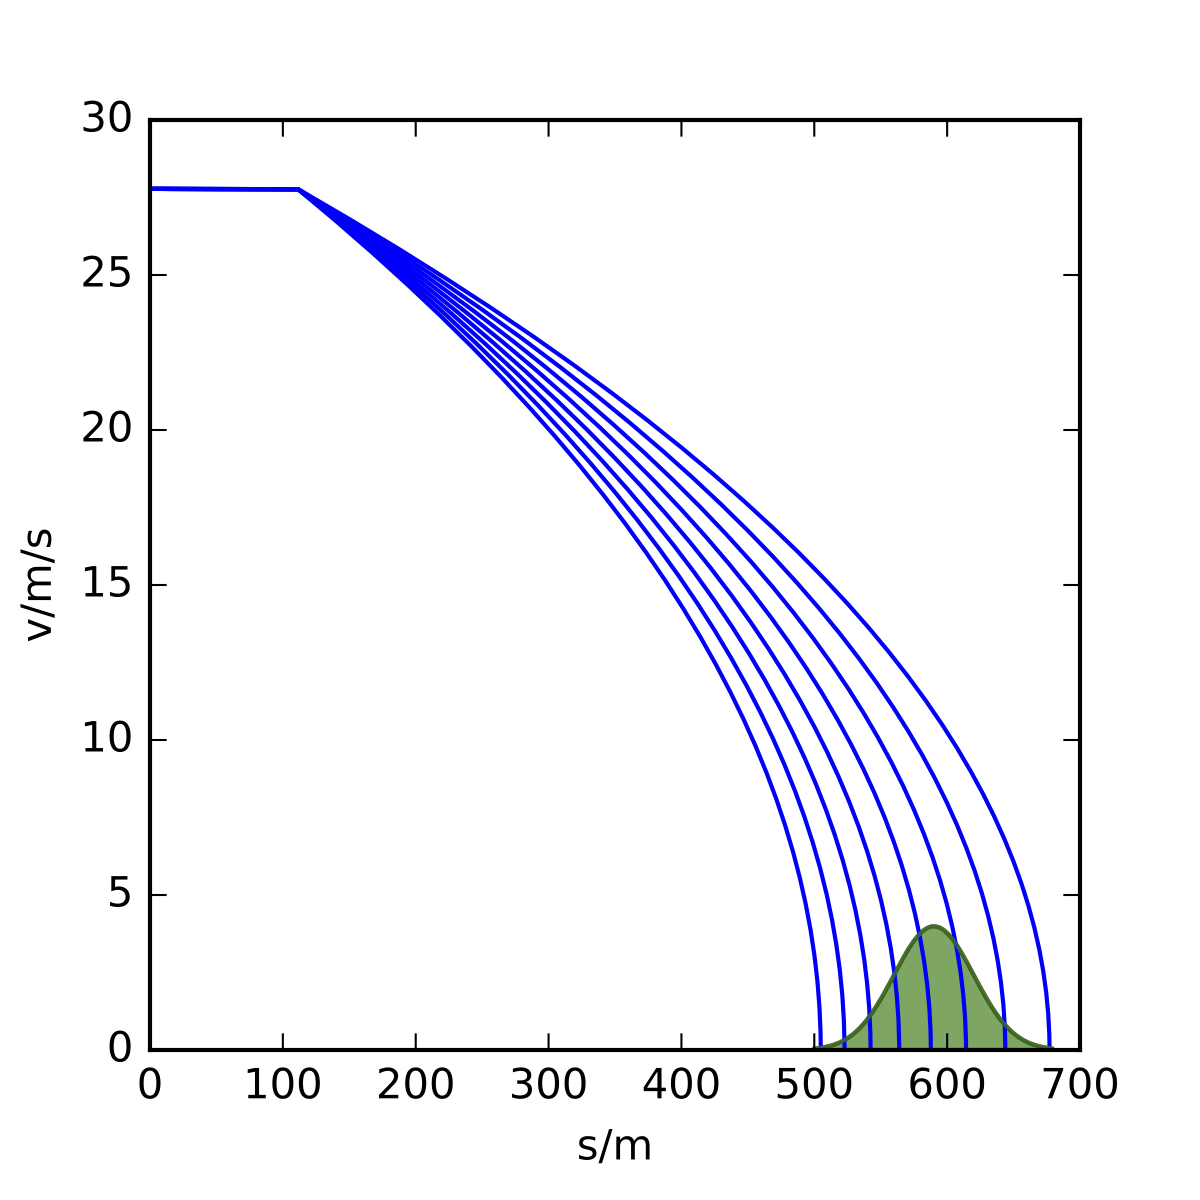
\includegraphics[scale=0.2]{./pic/171026_Transrail_BrakingCurves-14}
	\caption{Braking curves \cite{Pfaff2017}}
	\label{fig:brakingcurves}
\end{figure}

\section{Problem}
\label{sec:Problem}

\par\noindent
As mentioned, one category of input parameters for the calculation of braking curves is data directly associated with the rolling stock, and in particular to the braking system itself. While this does not necessarily present itself as an issue in passenger trains, freight wagons, in contrast, are usually not electrified and therefore do not currently posses the sensory equipment that would be necessary to obtain such data in an adequate quantity and quality, especially in regards to \textit{big data processing}. Although it has been proposed to equip freight wagons accordingly (Refer to the concept \enquote{freight wagon 4.0} by Dr. Manfred Enning and Dr. Raphael Pfaff \cite{Enning2017}), it will be years, possibly decades, before enough rolling stock has been retrofitted as to make it possible to obtain the desired data. Since braking curves vary according to the rolling stock, this lack of data makes calculation thereof impossible.

\section{Solution}
\label{sec:Solution}

\par\noindent
Since the problem is lack of data from real life operations, this work proposes to circumvent this by generation of artificial, simulated data instead. The data set should replicate the actual distribution of braking behavior as closely as possible. It is therefore necessary to first create a model encompassing the braking process of a freight train. This model will be discussed in depth in chapter \ref{chap:ModelingOfTrainOperations}. By using that model to run a large number of simulated braking processes, one may obtain data about the behavior of the braking system, which, albeit being artificial, should at least satisfy requirements for the calculation of rudimentary braking curves. A freely configurable simulation environment further allows for great flexibility in terms of input parameters, therefore enabling for covering a very large range of data, where computing power and time are the only limiting factors. The process of data generation and simulation will be discussed further in chapter \ref{chap:DataGeneration}.
\par
As real life operations would yield very high quantities of data, the simulation output must be stored in a data structure which is suitable for big data processing. This structure will also be discussed in chapter \ref{chap:DataGeneration}.
\chapter{Fundamentals of Railway Vehicle Engineering}
\label{chap:FundamentalsOfRailwayVehicleEngineering}
\par\noindent
\textit{\textbf{Introduction}} This section deals with the engineering backgrounds of the work, especially in regards to railway vehicle engineering and railway physics. 
For the creation of a braking model, it is necessary to have at least a basic understanding of the engineering and physics behind rail traffic. The most fundamental component to understand is, of course, the actual braking process.

\section{The Train Brake}
\label{sec:TrainBrake}
\par\noindent
There are a number of different construction methods for brakes, but each must address two problems: The means of transmission of commands and the actual form of brake force generation. The focus here will lie on the pneumatic brake, since it is still the most prevalent in cargo vehicles. From a macro perspective, the pneumatic brake has three main components: The train driver's brake valve, the brake pipe and one or more brake cylinders for each wagon or locomotive. The driver's valve and the brake pipe are primarily the means of command transmission, while the brake cylinder's job is the generation of brake force. 

\par
The braking system is an indirect one, which means the brake pipe needs to be vented to apply the brakes. Therefore, the brake pipe is kept at a running pressure of 5 bar. One advantage of this approach is that brakes are automatically applied in case of train separation. The downside, however, is that command transmission is limited to the speed of sound. In order to generate that pressure, the locomotive contains a compressor and an air reservoir. Initially, the brake pipe as well as all auxiliary air reservoirs are brought to operating pressure. If the train operator wishes to brake, he has to actuate the driver's brake valve, which in turn vents the brake pipe, usually as far as 3.5 bar (full braking), sometimes even lower. As rule of thumb, the more pressure is vented, the more braking force is applied. Each wagon brake has, in essence, an auxiliary air reservoir, a distributor valve and a braking cylinder. When the brake pipe is vented, the air in the auxiliary reservoir has a higher pressure. This difference in pressure triggers a switch of the distributor valve, and the air from the reservoir may go into the brake cylinder. This increase in the cylinder generates the actual braking force. To summarize, the amount of generated braking pressure is directly proportional to the amount of pressure vented.

\section{Influences on Braking Performance}
\label{sec:InfluencesOnBraking}
\par\noindent
Since the aim of this work is to monitor braking performance, it becomes necessary to understand which factors influence the braking process, and how. The braking process is, in its core, a system. A system may be defined as a set of objects, which are interconnected by relations. It is enclosed by its environment, which may or may not affect the system itself. Below is an illustration, also called box model:

\begin{align*}
	\displaystyle {\mathcal {R}}\ 
	\rightarrow \ 
	{\begin{array}{|c|}\hline \quad \\\quad {\mathcal {V}}_{i}\leftrightarrow {\mathcal {V}}_{n}\quad \\\quad \\\hline \end{array}}\ 
	\rightarrow
\end{align*}

\par\noindent
The box represents the actual system, ${\mathcal{V}}_{i}$ are the system variables, or objects, their relations represented by the $\leftrightarrow$. The ${\mathcal{R}}$ represents the system's environment and its influence on the system itself. Finally, the rightmost arrow $\rightarrow$ is the influence the system might have on the environment, though this is often disregarded as the focus lies on what happens inside the system. Creating a box model for the braking process makes for an easier identification of the influencing factors, and allows for their categorization into inherent, i.e. system variables, and external, i.e. system environment.
\par
From a modeling perspective, it is sensible to differentiate as follows: Everything related to the train itself is part of the system, and everything else is part of the system's environment. As per definition, it is compromised of a set of variables, a set of relations, and a set of constants. Let us make a formal definition of the model for the braking process system:

\begin{align*}
{\mathcal {M}} = \{ {\mathcal{V}}, {\mathcal{R}}, {\mathcal{C}} \}
\end{align*}

\noindent
where ${\mathcal{V}}$ is the set of system variables, ${\mathcal{R}}$ is the set of relations (a) between elements of ${\mathcal{V}}$ and (b) between system and environment, and ${\mathcal{C}}$ is the set of system constants. The system variables may be subsystems themselves. We shall take a closer look at ${\mathcal{V}}$ first.

\subsection{Inherent factors, model variables}
\label{sec:InherentFactors}
\par\noindent
Looking at ${\mathcal{M}}$, which is the system describing the braking process, ${\mathcal{V}}$ consists of all factors inherent to the train which have an impact on the braking, as well as the relevant quantifiers. The main ones are:
\begin{itemize}
	\item The train brake
	\item The wagon mass, denoted as $m$
	\item The train velocity, denoted as $v$
	\item The train composition, i.e. in which order the wagons are, for example the heaviest wagons being in front and the lighter ones at the back, denoted as $comp$
	\item The generated braking force, denoted as $F_{b}$
	\item The train's deceleration, denoted as $a$
	\item The train's braking distance, denoted as $d$
\end{itemize}
\noindent
It is noteworthy that the train brake is another system in itself, which is perfectly fine of course. Alas, it is therefore necessary to define another model.

\begin{align*}
{\mathcal {M}}_{B} = \{ {\mathcal {V}}_{B}, {\mathcal {R}}_{B}, {\mathcal {C}}_{B} \}
\end{align*}

\noindent
Let ${\mathcal{M}}_{B}$ be the model describing the system train brake, with ${\mathcal {V}}_{B} = \{ {\mathcal {M}}_{bv}, {\mathcal {M}}_{bp}, {\mathcal {M}}_{bc} \}$, where ${\mathcal {M}}_{bv}$ is the model of the brake valve, ${\mathcal {M}}_{bp}$ the model of the brake pipe and ${\mathcal {M}}_{bc}$ the model of the brake cylinder, which in turn shall be defined as follows:

\begin{align*}
{\mathcal {M}}_{bv} = \{ {\mathcal {V}}_{bv}, {\mathcal {R}}_{bv}, {\mathcal {C}}_{bv} \}
\end{align*}

\noindent
Let ${\mathcal {M}}_{bv}$ be the model describing the system brake valve, with ${\mathcal {V}}_{bv} = \{x\}$, ${\mathcal {R}}_{bv} = \emptyset$ and $c_{bv} = \emptyset$, where $x$ is the state of the brake valve, i.e. its opening percentage, ranging from 0 (fully closed) to 1 (fully open, full braking).

\begin{align*}
{\mathcal {M}}_{bp} = \{ {\mathcal {V}}_{bp}, {\mathcal {R}}_{bp}, {\mathcal {C}}_{bp} \}
\end{align*}

\noindent
Let ${\mathcal {M}}_{bp}$ be the model describing the system brake pipe, with ${\mathcal {V}}_{bp} = \{ l_{bp}, p_{bp} \}$, ${\mathcal {R}}_{bp} = \emptyset$ and $c_{bp} = \{ v_{bp} \}$, where $l_{bp}$ is the physical length of the brake pipe, $p_{bp}$ is the pressure on the brake pipe and $v_{bp}$ is the propagation velocity of the pipe's medium. 

\begin{align*}
{\mathcal {M}}_{bc} = \{ {\mathcal {V}}_{bc}, {\mathcal {R}}_{bc}, {\mathcal {C}}_{bc} \}
\end{align*}

\noindent
Let ${\mathcal {M}}_{bc}$ be the model describing the system brake cylinder, with ${\mathcal {V}}_{bc} = \{ p_{bc} \}$, ${\mathcal {R}}_{bc} = \emptyset$ and $c_{bc} = \{ t_{bc} \}$, where $p_{bc}$ is the cylinder's pressure and $t_{bc}$ is the cylinder's fill time.
\bigskip
\par\noindent
This wraps up the definition of ${\mathcal{V}}_{B}$. We may now get to the definition of ${\mathcal{R}}_{B}$, which consists of the relations (a) between the elements of ${\mathcal{V}}_{B}$ and (b) between ${\mathcal{M}}_{B}$ and its environment. Let us begin with (a):
\bigskip
\par\noindent
\textit{\textbf{Convention}} For readability purposes, $\propto$ shall from here on denote direct proportionality, and $\sim$ shall denote inverse proportionality.
\bigskip
\par
${\mathcal{M}}_{bv}$ relates to ${\mathcal{M}}_{bp}$ in the sense that the state of the brake valve has a direct influence on the pressure on the brake pipe. More specifically, $x \in {\mathcal{V}}_{bv}$ is inversely proportional to $p_{bp} \in {\mathcal{V}}_{bp}$. The higher the value of $x$, i.e. the opening percentage of the brake valve, the lower the value of $p_{bp}$, i.e. the pressure on the brake pipe. We can therefore denote $x \sim p_{bp}$, and subsequently define a relation $R_{bv,bp}: {\mathcal{M}}_{bv} \sim {\mathcal{M}}_{bp}$. 
\par
${\mathcal{M}}_{bp}$ relates to ${\mathcal{M}}_{bc}$ in the sense that the pressure on the brake pipe has a direct influence on the brake cylinder's pressure. More specifically, $p_{bp} \in {\mathcal{V}}_{bp}$ is inversely proportional to $p_{bc} \in {\mathcal{V}}_{bc}$. The lower the value of $p_{bp}$, i.e. the pressure on the brake pipe, the higher the value $p_{bc}$, i.e. the pressure in the brake cylinder. We can therefore denote $p_{bp} \sim p_{bc}$, and subsequently define a relation $R_{bp,bc}: {\mathcal{M}}_{bp} \sim {\mathcal{M}}_{bc}$.
\par
For simplicity, we can look at ${\mathcal{M}}_{B}$ as being isolated from its environment, i.e. the environment does not impact ${\mathcal{M}}_{B}$, and vice versa. Therefore, (b) is void. Consequently, we can define ${\mathcal{R}}_{B}$ as follows:

\begin{align*}
{\mathcal{R}}_{B} = \{ R_{bv,bp}, R_{bp,bc} \}
\end{align*}

\noindent
This finally leaves us with $c_{B}$. Since call constants are specific to the respective sub-models $\in {\mathcal{V}}_{B}$, ${\mathcal{M}}_{B}$ has no constants of its own, therefore $c_{B} = \emptyset$. This completes the definition of ${\mathcal{M}}_{B}$, and we can properly define the set of model variables of the model braking process:

\begin{align*}
{\mathcal{V}} = \{ {\mathcal{M}}_{B},m,v,comp,F_{b},a,d \}
\end{align*}

\subsection{Relations}
\label{sec:Relations}
\par\noindent
Looking at our model ${\mathcal{M}}$, we have now defined its set of variables, ${\mathcal{V}}$. Next, it is necessary to define its set of relations, ${\mathcal{R}}$, which may be distinguished into internal and external relations.

\subsubsection{Relations between system variables}
\label{sec:RelationsSystemVariables}
\par\noindent
Obviously, the train brake ${\mathcal{M}}_{B}$ relates to $F_{B}$ as it is the actor responsible for generating the braking force. More specifically, $p_{bc} \in {\mathcal{V}}_{bc}$, which is the pressure in the brake cylinder, is directly proportionate to $F_{b}$, meaning the higher the pressure, the more force is applied. We can therefore denote $p_{bc} \propto F_{b}$, and subsequently define a relation $R_{{\mathcal{M}}_{B},F_{b}}: {\mathcal{M}}_{B} \propto F_{b}$.
\par
Furthermore, the wagon mass $m$ relates to $F_{B}$ as well. The vehicle mass is proportional to the kinetic energy to dissipate during braking actions. The larger $m$ is, the more kinetic energy ($E=\frac{1}{2} \cdot m \cdot v^{2}$), and thus the higher the required braking force to slow the train down. As the vehicle mass varies, so must the applied braking force in order to avoid wheel slip and locking of the wheels which occurs if too much force is applied (\cite{Cruceanu2012}, p.47). We can therefore denote $m \propto F_{b}$, and subsequently define a relation $R_{m,F_{b}}: m \propto F_{b}$.
\par
The braking deceleration $a$, neglecting other resistances, is influenced by two factors: The applied braking force $F_{b}$, and the vehicle's mass $m$. As per Newton's second law of motion, $F=m \cdot a$, so $a=\frac{F_{b}}{m}$ (\cite{Cruceanu2012}, p.51). In practice, this means the braking force is directly proportional to the braking deceleration, and the vehicle mass is inversely proportional to $a$, not taking into consideration wheel slip. We can therefore denote $F_{b} \propto a$, and $m \sim a$, and subsequently define two relations $R_{F_{b},a}: F_{b} \propto a$, and $R_{m,a}: m \sim a$.
\par
Finally, the braking distance $d$ is also dependent on two factors: The running speed $v$, and the braking deceleration $a$.  We have 

\begin{equation}
\label{eq:brakingdistance}
\begin{aligned}
&d=\frac{1}{2} \cdot a \cdot t^{2} \\
&v=a \cdot t \quad \rightarrow \quad d=\frac{v^{2}}{2 \cdot a}
\end{aligned}
\end{equation}

\noindent
where $t$ is the stopping time (\cite{Cruceanu2012}, p.51). So in practice, the square of the running speed $v$ is directly proportional to the braking distance, and the braking deceleration is inversely proportional to $d$. We can therefore denote $v \propto d$, and $a \sim d$, and subsequently define two relations $R_{v,d}: v \propto d$, and $R_{a,d}: a \sim d$.
\par
This completes the set of internal relations of ${\mathcal{R}}$.

\subsubsection{Relations between environment and system}
\label{sec:RelationsEnvironmentSystem}
\par\noindent
To recapitulate, ${\mathcal{M}}$ is a model for the braking process. Having handled its internal relations, it is now time to focus on the relation between the system and its environment. As established in section \ref{sec:InfluencesOnBraking}, the environment consists of all factors which have an influence on the braking process, but are not inherent to the train itself. In practice, this is the track which the train operates on. More specifically, it is two main properties of the track:
\begin{itemize}
	\item The track gradient, denoted as $\alpha$
	\item The wheel/rail friction coefficient, denoted as $\mu$
\end{itemize}
\noindent
As shown earlier, the braking deceleration has a substantial influence on the braking process, namely on the braking distance and on the stopping time (see equation \ref{eq:brakingdistance}). So far, the deceleration was only related to vehicle mass $m$ and applied braking force $F_{b}$, both being internal relations. However, the track gradient also has an influence on $a$. As the train goes uphill, the deceleration increases; as it goes downhill, it decreases, due to gravity. A simple formula might look like this:

\begin{equation}
\label{eq:deceleration}
a = a_{brake} + a_{grad}
\end{equation}

\noindent
where $a$ is the total braking deceleration, $a_{brake}$ is the deceleration resulting from the application of the brakes, and $a_{grad}$ is the acceleration/deceleration resulting from the track gradient. Let $a_{grad}$ be positive for upward, negative for downward slopes. We can define $a_{grad}$ as a step function

\begin{equation}
\label{eq:gradientdeceleration}
a_{grad}(\alpha) =
\begin{cases}
\geq 0 & \text{if $\alpha \geq 0$} \\
< 0 & \text{if $\alpha < 0$}
\end{cases}
\end{equation}

\noindent
where $\alpha$ is the value of the gradient, e.g. a percentage or an angle. This shows the track gradient is directly proportional to the total braking deceleration. We can therefore denote $\alpha \propto a$, and subsequently define a relation $R_{\alpha,a}: \alpha \propto a$.
\par
The second factor to look at is the wheel/rail adhesion. Environmental effects like rain, ice or contaminants such as leaves have a degrading effect on the wheel/rail friction. This is expressed by a friction coefficient $\mu$, where a lower value, for example $\mu = 0.2$ for a wet rail surface, means worse braking performance compared to a higher value, e.g. $\mu = 0.4$ for normal conditions. The friction coefficient is a limiting factor for the applied braking force, in the sense that when too much force force is applied, wheel slip occurs, and braking performance decreases (\cite{Bosso2006}, p.876). While $\mu$ does not have a direct influence on $F_{b}$, it is, in practice, still related to it in that it is a limiting factor; an indirect influence, so to speak. In that regard, we might say it is directly proportional to the braking force: The higher the friction coefficient, the higher the maximum braking force that may be applied. We can therefore denote $\mu \propto F_{b}$, and subsequently define a relation $R_{\mu,F_{b}}: \mu \propto F_{b}$.
\bigskip
\par\noindent
We may now properly define the set of relations of the model braking process:

\begin{align*}
{\mathcal{R}} = \{ R_{{\mathcal{M}}_{B},F_{b}} \:,\: R_{m,F_{b}} \:,\: R_{F_{b},a} \:,\: R_{m,a} \:,\: R_{v,d} \:,\: R_{a,d} \:,\: R_{\alpha,a} \:,\: R_{\mu,F_{b}} \}
\end{align*}

\section{Constants}
\label{sec:Constants}
\par\noindent
The braking process, being a dynamic one, has no constants in itself. Some of its components do, in particular the models making up the train brake, like the brake pipe ${\mathcal{M}}_{bp}$'s propagation velocity $v_{bp}$. However, these have already been discussed; we can therefore conclude that ${\mathcal{C}} = \emptyset$.
\bigskip
\par\noindent
To summarize, we have now defined all necessary components of ${\mathcal{M}}$, namely its set of model variables ${\mathcal{V}}$, its set of relations ${\mathcal{R}}$, and its set of constants ${\mathcal{C}}$. This model will be used in chapter \ref{chap:ModelingOfTrainOperations} as a theoretical basis upon which to build a Simulink model, simulating the braking process.

\section{Time considerations}
\label{sec:TimeConsiderations}
\par\noindent
So far, we have looked at the braking process from a static point of view. However, in reality it is a dynamic process and thus, time has to be taken into consideration. More specifically, it is a continuous model: For ${\mathcal{M}}$, the state of its variables changes all the time for the whole duration of the process. 
\par
Remember how we have defined the model. It is a set comprising of a number of subsets; but it describes a system, in this case the braking process of a train. This means that the model variables, i.e. the elements of ${\mathcal{V}}$, are subject to change as the process progresses. This can be expressed by another equation, in form of a function $f$:

\begin{align*}
{\mathcal{V}} &= f( {\mathcal{M}} ) \\
		&= f( {\mathcal{V}}, {\mathcal{R}}, {\mathcal{C}} )
\end{align*}

\noindent
This suffices to determine the system's state before and after a relation has changed. As an example, $v$ might be $25 \; \frac{m}{s}$ when the train operator engages the brakes, and $10 \; \frac{m}{s}$ when the brakes have been released. However, since we wish to monitor the whole braking process, it is also interesting to see how the state changes over time. In this example, $v$ would be $25 \; \frac{m}{s}$ for $t=0$, $22.3 \; \frac{m}{s}$ for $t=50$ etc. We therefore need a new equation where ${\mathcal{V}}$ is also dependent on $t$.

\begin{align*}
{\mathcal{V}}(t)' = f ( {\mathcal{M}} )
\end{align*}

\noindent
This allows for the calculation of the rate of change for any given point in time. By integrating the equation, one can also obtain the actual values of the elements of ${\mathcal{V}}$, e.g. the value of $v$ for $t=120$. The function $f$ is one, or a set of, differential equations. In practice, these are automatically generated and calculated by Simulink, so we need not be concerned with their exact definition at this point.
\bigskip
\par\noindent
We have now laid all the necessary groundwork to build a functioning model of the braking process, which can then be used for simulation and data generation. The next chapter will deal with this.
\chapter{Modeling of Train Operations}
\label{chap:ModelingOfTrainOperations}
\par\noindent
\textit{\textbf{Introduction}} Chapter \ref{chap:FundamentalsOfRailwayVehicleEngineering} has established the theoretical model of the train braking process. It will serve as a foundation to build a practical model suitable for conducting actual simulations. 

\section{Matlab Simulink}
\label{sec:MatlabSimulink}
The model has been built utilizing the software Matlab Simulink by Mathworks. It offers several distinct advantages: It uses a graphical block diagramming tool which makes it very intuitive to use. At the same time, various official and third-party add-on libraries make it very versatile. Most importantly, as it is tightly integrated with the Matlab environment, it can be used for both modeling and simulating dynamical systems, like the braking process of a train.

\section{Initial Model}
\label{sec:InitialModel}
\par\noindent
Looking back at chapter \ref{chap:FundamentalsOfRailwayVehicleEngineering}, the aim is to build a model for the braking process of a freight train. An initial model of a single braking procedure, kindly provided by Dr. Raphael Pfaff, will serve as a basis. Most of the components previously designed in chapter \ref{chap:FundamentalsOfRailwayVehicleEngineering} can already be found therein.  

\begin{figure}[H]
	\centering
	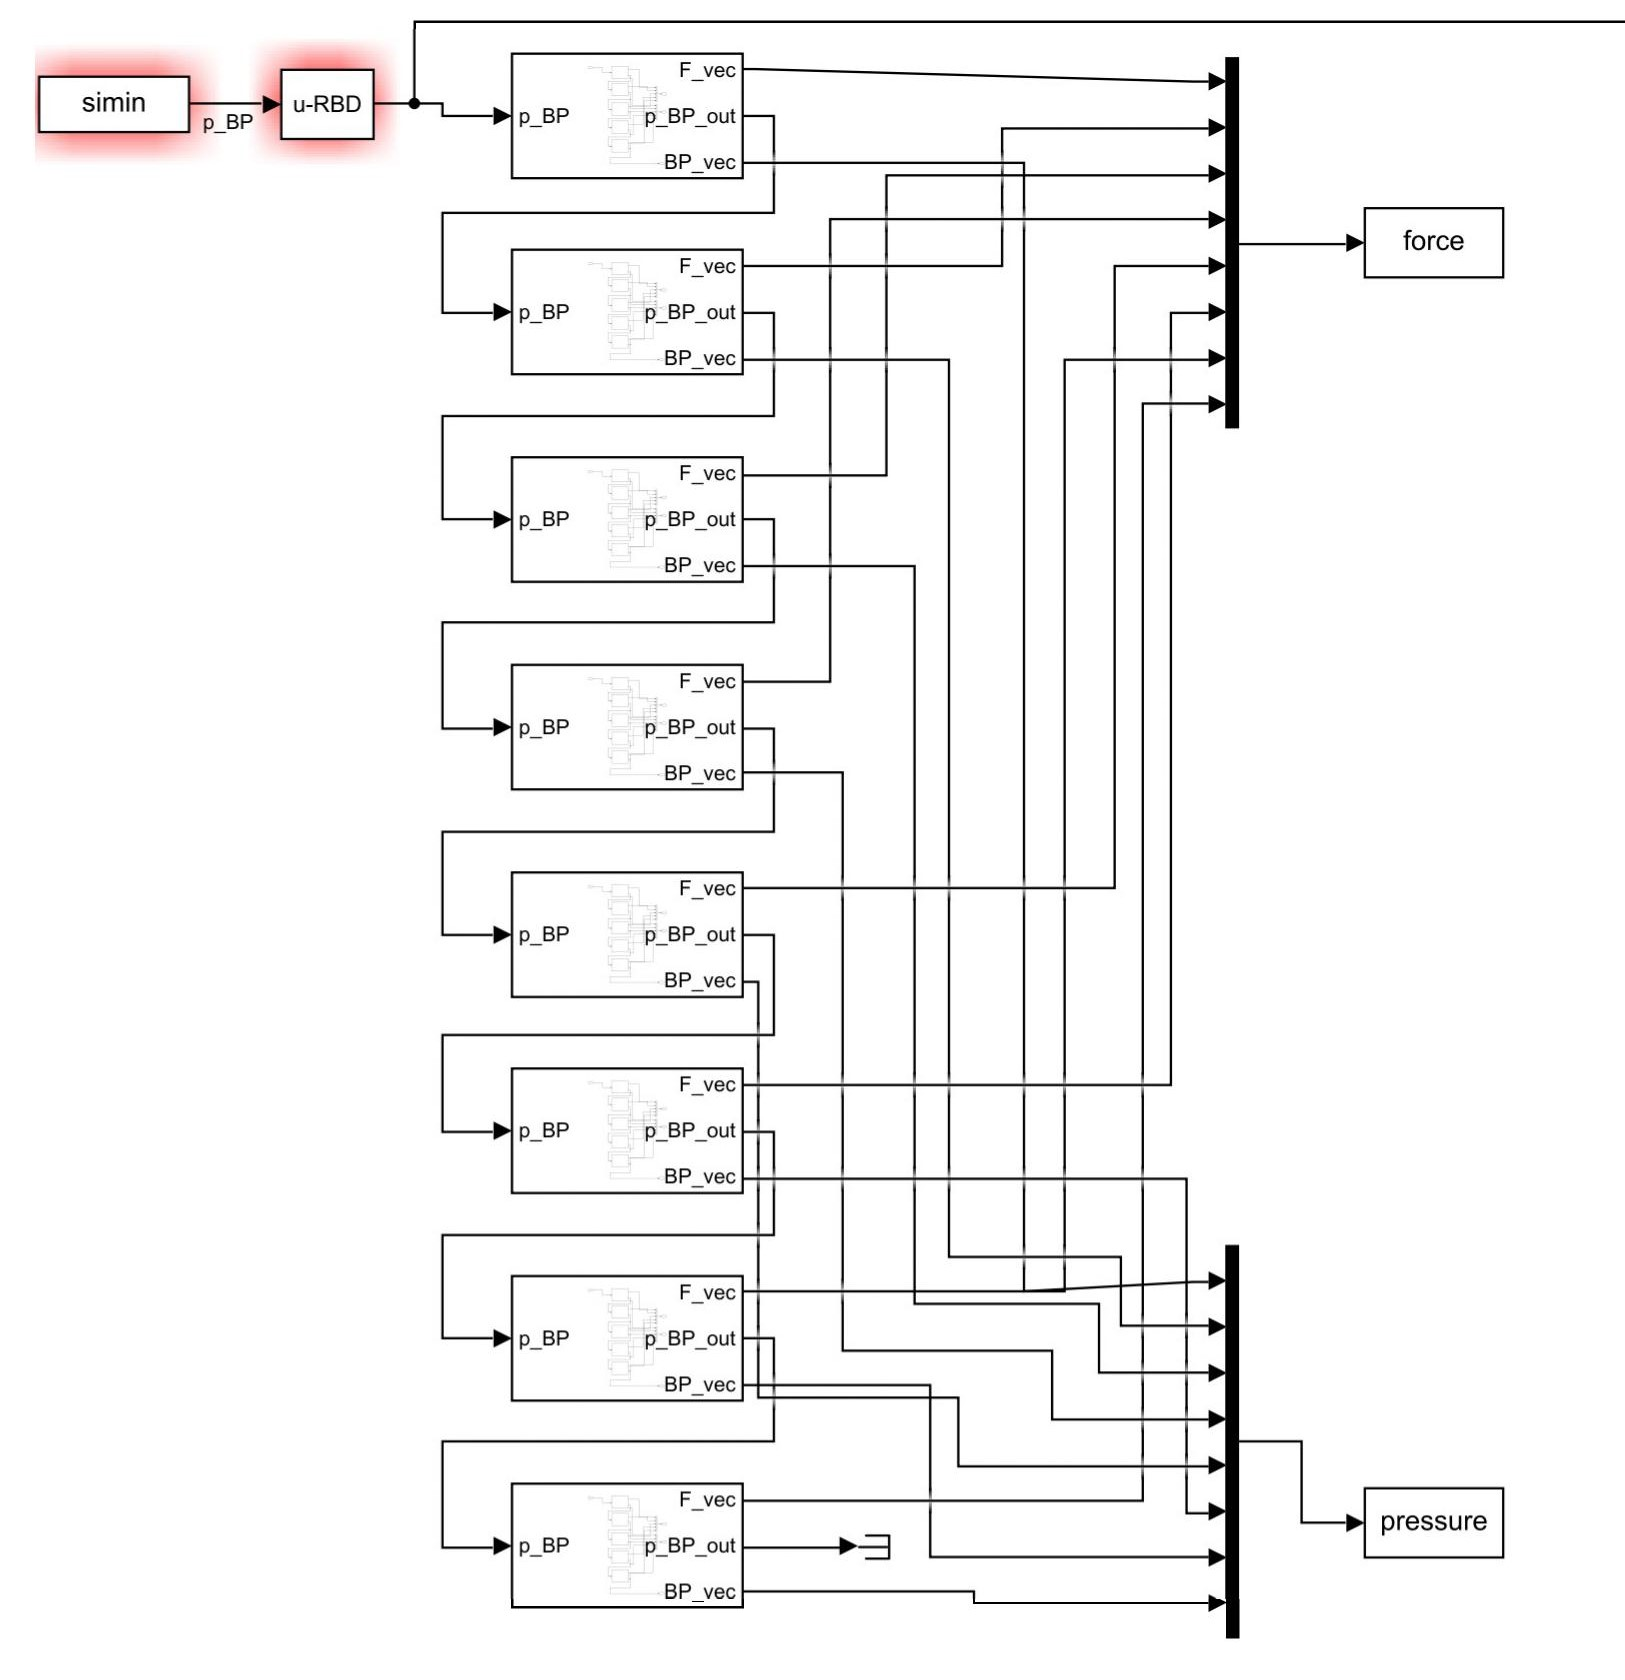
\includegraphics[width=\linewidth]{./pic/initmodel_whole}
	\caption{Initial Model}
	\label{fig:initmodel_whole}
\end{figure}

\par\noindent
Figure \ref{fig:initmodel_whole} shows a model of a freight train of fixed length, consisting of 40 wagons in total. For better readability, five wagons are condensed into one subsystem each, marked by the red rectangle. The subsystems are interconnected by a brake pipe, marked by the green arrow. They have one input port for the incoming pressure on the brake pipe, and three output ports, one for the pipe connection to the next subsystem, and two for recording brake pressure and brake force (marked by the pink and blue arrows, respectively). A depiction of a subsystem can be found in appendix \ref{fig:initmodel_subsys}.  

\begin{figure}[H]
	\centering
	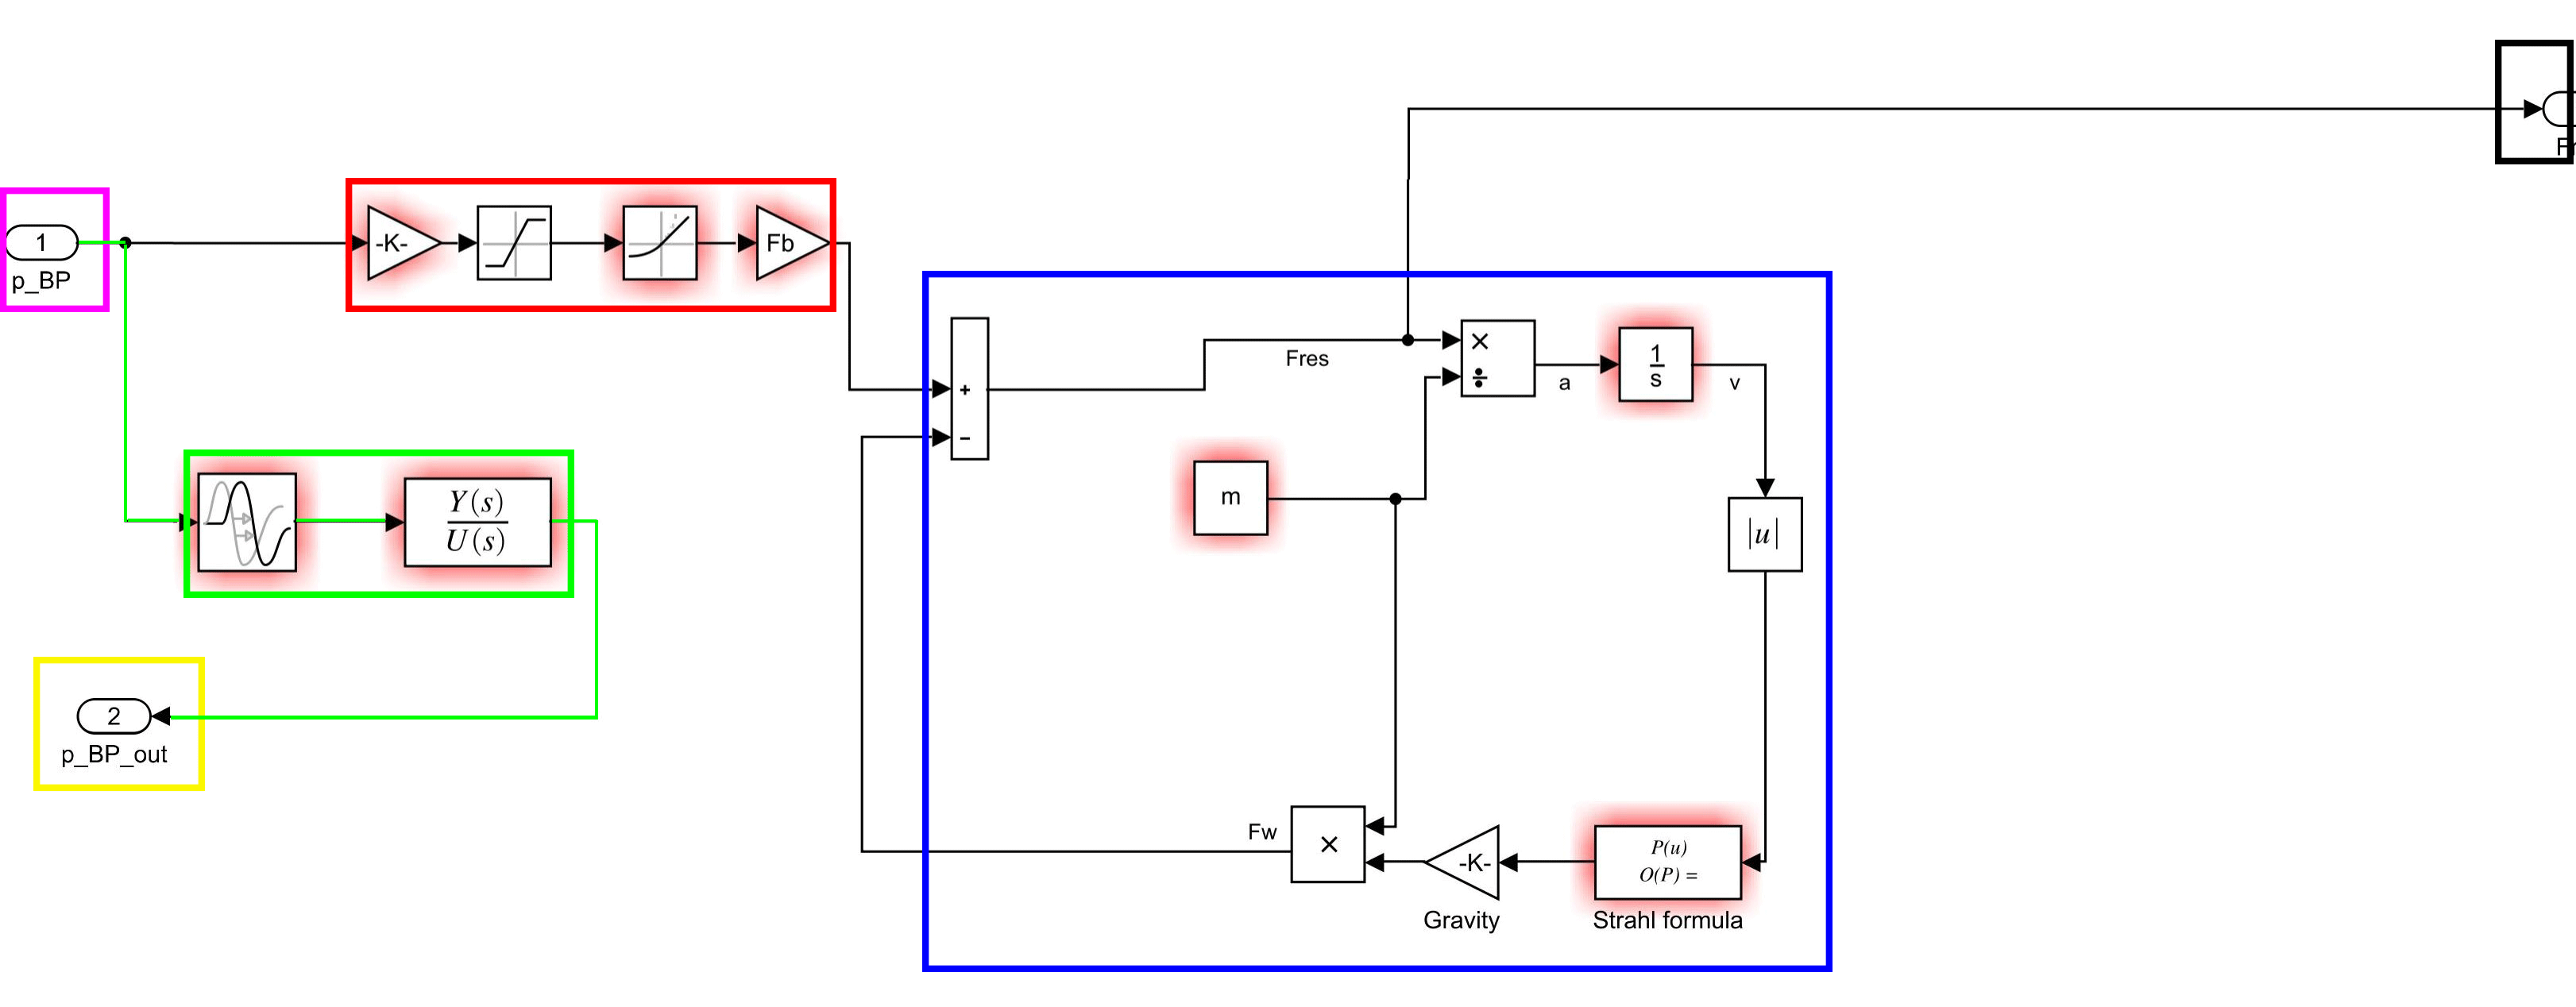
\includegraphics[width=\linewidth]{./pic/initmodel_wagon}
	\caption{Initial Model - Wagon}
	\label{fig:initmodel_wagon}
\end{figure}

\par\noindent
Figure \ref{fig:expandedmodel_wagon} shows a model of a freight wagon. It already encompasses several of the model variables defined in section \ref{sec:InherentFactors}. The brake pipe ${\mathcal{M}}_{bp}$ is represented by the green arrows. It leads from input port (pink rectangle) to output port (yellow rectangle); the propagation delay is realized by a transport delay block (green rectangle), using propagation velocity $v_{bp}$ and wagon length $l_{bp}$. The brake pressure $p_{bp}$ is the value of the signal traveling through the connection. Note that in the simulation, the signal value for $p_{bp}$ is the difference between regular operating pressure and actual pressure, e.g. if simulated pressure on the brake pipe is 3.5 bar, the signal value is $3.5 - 5 = -1.5$.
\par
The brake cylinder ${\mathcal{M}}_{bc}$ is represented by the red rectangle. The pressure on the brake pipe $p_{bp}$ is converted into a coefficient between zero and one, where zero equals no brakes applied, or $p_{bp} = 5$, and one equals full braking pressure, or $p_{bp} = 3.5$. The exact formula is this:

\begin{align*}
p_{bc} = p_{bp} \cdot \frac{-1}{5-3.5}
\end{align*}

\noindent
So for a braking pressure of 4 bar, the coefficient would be $(4 - 5) \cdot \frac{-1}{5-3.5} = -1 \cdot \frac{-1}{1.5} = \frac{2}{3}$. A rate limiter block accounts for the brake cylinder's filling time $t_{bc}$. Finally, the braking force is calculated by multiplying the maximum braking force, which is mainly dependent on the wagon mass $m$ [train braking, 22]. So for the braking pressure, we have:

\begin{align*}
F_{b} = F_{b,max} \cdot p_{bc}
\end{align*}

\noindent
The final component is the factoring in of the driving resistance of the train, utilizing Strahl's formula. This is represented by the blue rectangle. By continuous-time integration of the acceleration, which is calculated according to Newton's second law of motion ($a = \frac{F}{m})$, it is possible to determine the velocity, which in turn allows for the calculation of the force generated by the driving resistance, This force is then added to the braking force and fed into an output port, marked with the black rectangle.
\par
Regarding simulation, this initial model is only fit for one single braking process, where a train of fixed length and fixed composition, brakes from an initial velocity all the way to a halt; the only variation is the pressure on the brake pipe, which is also the sole input for the simulation. Appendix \ref{fig:initmodel_input} shows how that input might look like.

\section{Model Expansion}
\label{sec:ModelExpansion}

\par\noindent
This initial model is however not of sufficient detail. Where it merely simulates a single, rather undynamic braking process, the goal is the simulation of a train ride, with alternating phases of braking and accelerating. The model should furthermore factor in more components of the theoretical model ${\mathcal{M}}$ discussed in chapter \ref{chap:FundamentalsOfRailwayVehicleEngineering}, as well as allow for the recording of more properties specific to the braking process. For that purpose, the model has to be expanded. The simulation input needs to be changed in order to allow for the simulation of a train ride. Previously, it being only one braking process, using braking pressure as input was the obvious choice. This will be replaced by a track profile, according to which the train either engages its brakes, or accelerates. This will be discussed in further detail in chapter \ref{chap:DataGeneration}.
\par
In the initial model, the train is only able to decelerate by engaging its brakes. To allow for acceleration, it is necessary to expand the model accordingly. This may be realized by a rather simple two-point controller, which means the train is either accelerating or decelerating. The decision on whether to engage brakes or apply traction force at a particular point in time is made utilizing the track profile: If the current velocity of the train $v_{real}$ is greater than the maximum allowed velocity $v_{max}$ at that time, the train engages its brakes by lowering the pressure on the brake pipe $p_{bp}$. If $v_{real}$ is less than $v_{max}$, the train applies a traction force $F_{t}$ in order to increase speed. Both $p_{bp}$ and $F_{t}$ scale with the discrepancy between $v_{real}$ and $v_{max}$. This means the higher the value of $v_{dif}$ is, the more pressure is vented from the brake pipe (or the more traction force is applied). This prevents the train from overcompensating, for example applying full braking pressure to decrease velocity by $2 \; \frac{m}{s}$. Notice there is actually no case for when $v_{real}$ equals $v_{max}$, i.e. $v_{dif} = 0$. One might expect that this would lead to the train constantly oscillating between accelerating and decelerating, but in practice this does not occur, and it is thus unnecessary to account for that case.

\begin{figure}[H]
	\centering
	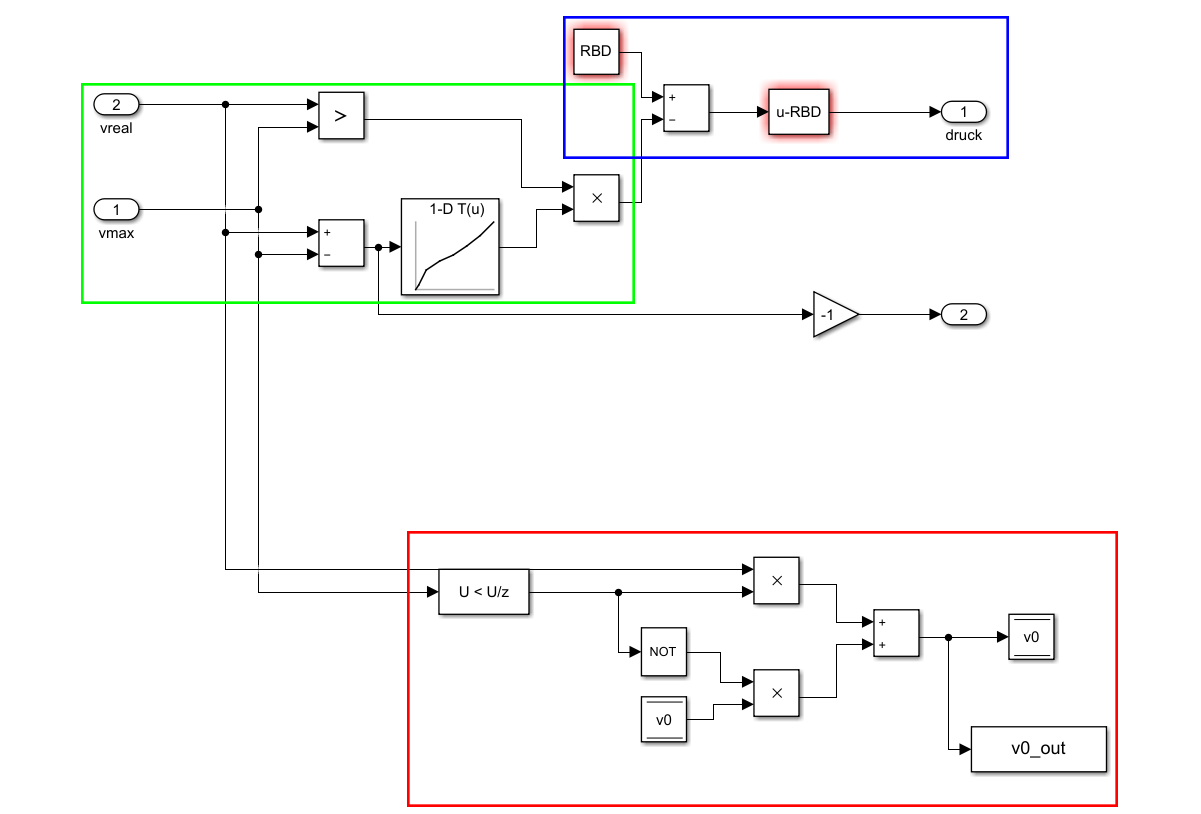
\includegraphics[width=\linewidth]{./pic/expandedmodel_pressure}
	\caption{Expanded Model - Pressure Calculation}
	\label{fig:expandedmodel_pressure}
\end{figure}

\par\noindent
Figure \ref{fig:expandedmodel_pressure} shows the subsystem responsible for the calculation of the braking pressure $p_{bp}$. The difference between $v_{real}$ and $v_{max}$ is used as input for a one-dimensional lookup table, which in essence is a step-function mapping different input values to discrete output values. 

\begin{equation}
\label{eq:lookuptable}
H(n) =
\begin{cases}
0.1 & \text{if $n=1$} \\
0.7 & \text{if $n=15$} \\
0.8 & \text{if $n=20$} \\
\text{..}
\end{cases}
\end{equation}

\noindent
Equation \ref{eq:lookuptable} is an example for how this function might look like. The input parameter $n$ stands for the discrepancy between actual and maximum velocity $v_{dif}$, and the output of the $H(n)$ represents the amount of pressure to vent from the brake pipe. This allows for adjusted braking, where $p_{bp}$ is directly proportional to $v_{dif}$.
\par
To account for the train only engaging its brakes in case its current velocity is higher than the maximum allowed velocity, a relational operator $>$ is used to compare $v_{real}$ to $v_{max}$.

\begin{equation}
\label{eq:brakingpressure}
P(n,t) = H(n) \cdot (v_{real}(t) > v_{max}(t))
\end{equation}

\noindent
Equation \ref{eq:brakingpressure} describes the logic. The braking pressure for a velocity discrepancy $n$ at a point in time $t$ equals the result of $H(n)$ (equation \ref{eq:lookuptable}) multiplied with the result of the relational operation comparing $v_{real}(t)$ to $v_{max}(t)$, which is 1 if $v_{real}(t)$ is greater than $v_{max}(t)$, and otherwise 0. This ensures that $P(n,t)$ is zero when the train's velocity is lower than the maximum allowed velocity, and thus no pressure is vented from the brake pipe, and no brakes are engaged. This part of the system is marked by the green rectangle in figure \ref{fig:expandedmodel_pressure}. The blue rectangle marks the conversion of the braking pressure into a signal fit for further calculations, analogous to the initial model, discussed previously. Finally, the red rectangle marks the component for storing the initial velocity of a braking process, which is needed to calculate the braking distance further down the line. This is achieved by using a block to detect a decrease of $v_{max}$, i.e. the block outputs a signal of 1 or 0, accordingly. 

\begin{equation}
\label{eq:initialvelocity}
v_{0} = v_{real} \cdot b + v_{0,old} \cdot \bar{b}
\end{equation}

\noindent
Equation \ref{eq:initialvelocity} describes the logic. The initial velocity of a braking process $v_{0}$ equals the train's velocity multiplied with the result of the decrease detection block, denoted as $b$, added with the previously stored initial velocity $v_{0,old}$ multiplied with the inverse of $b$, denoted as $\bar{b}$. If there is a decrease of $v_{max}$, i.e. the train starts braking, we get $v_{0} = v_{real} \cdot 1 + v_{0,old} \cdot 0 = v_{real}$. In any other case, we get $v_{0} = v_{real} \cdot 0 + v_{0,old} \cdot 1 = v_{0,old}$, i.e. the value of $v_{0}$ does not change as no new braking process has begun.
\par
This completes the description of this subsystem. It is worthy to note that, reaching back to chapter \ref{chap:FundamentalsOfRailwayVehicleEngineering}, this is the practical implementation of the brake valve ${\mathcal{M}}_{bv}$.

\begin{figure}[H]
	\centering
	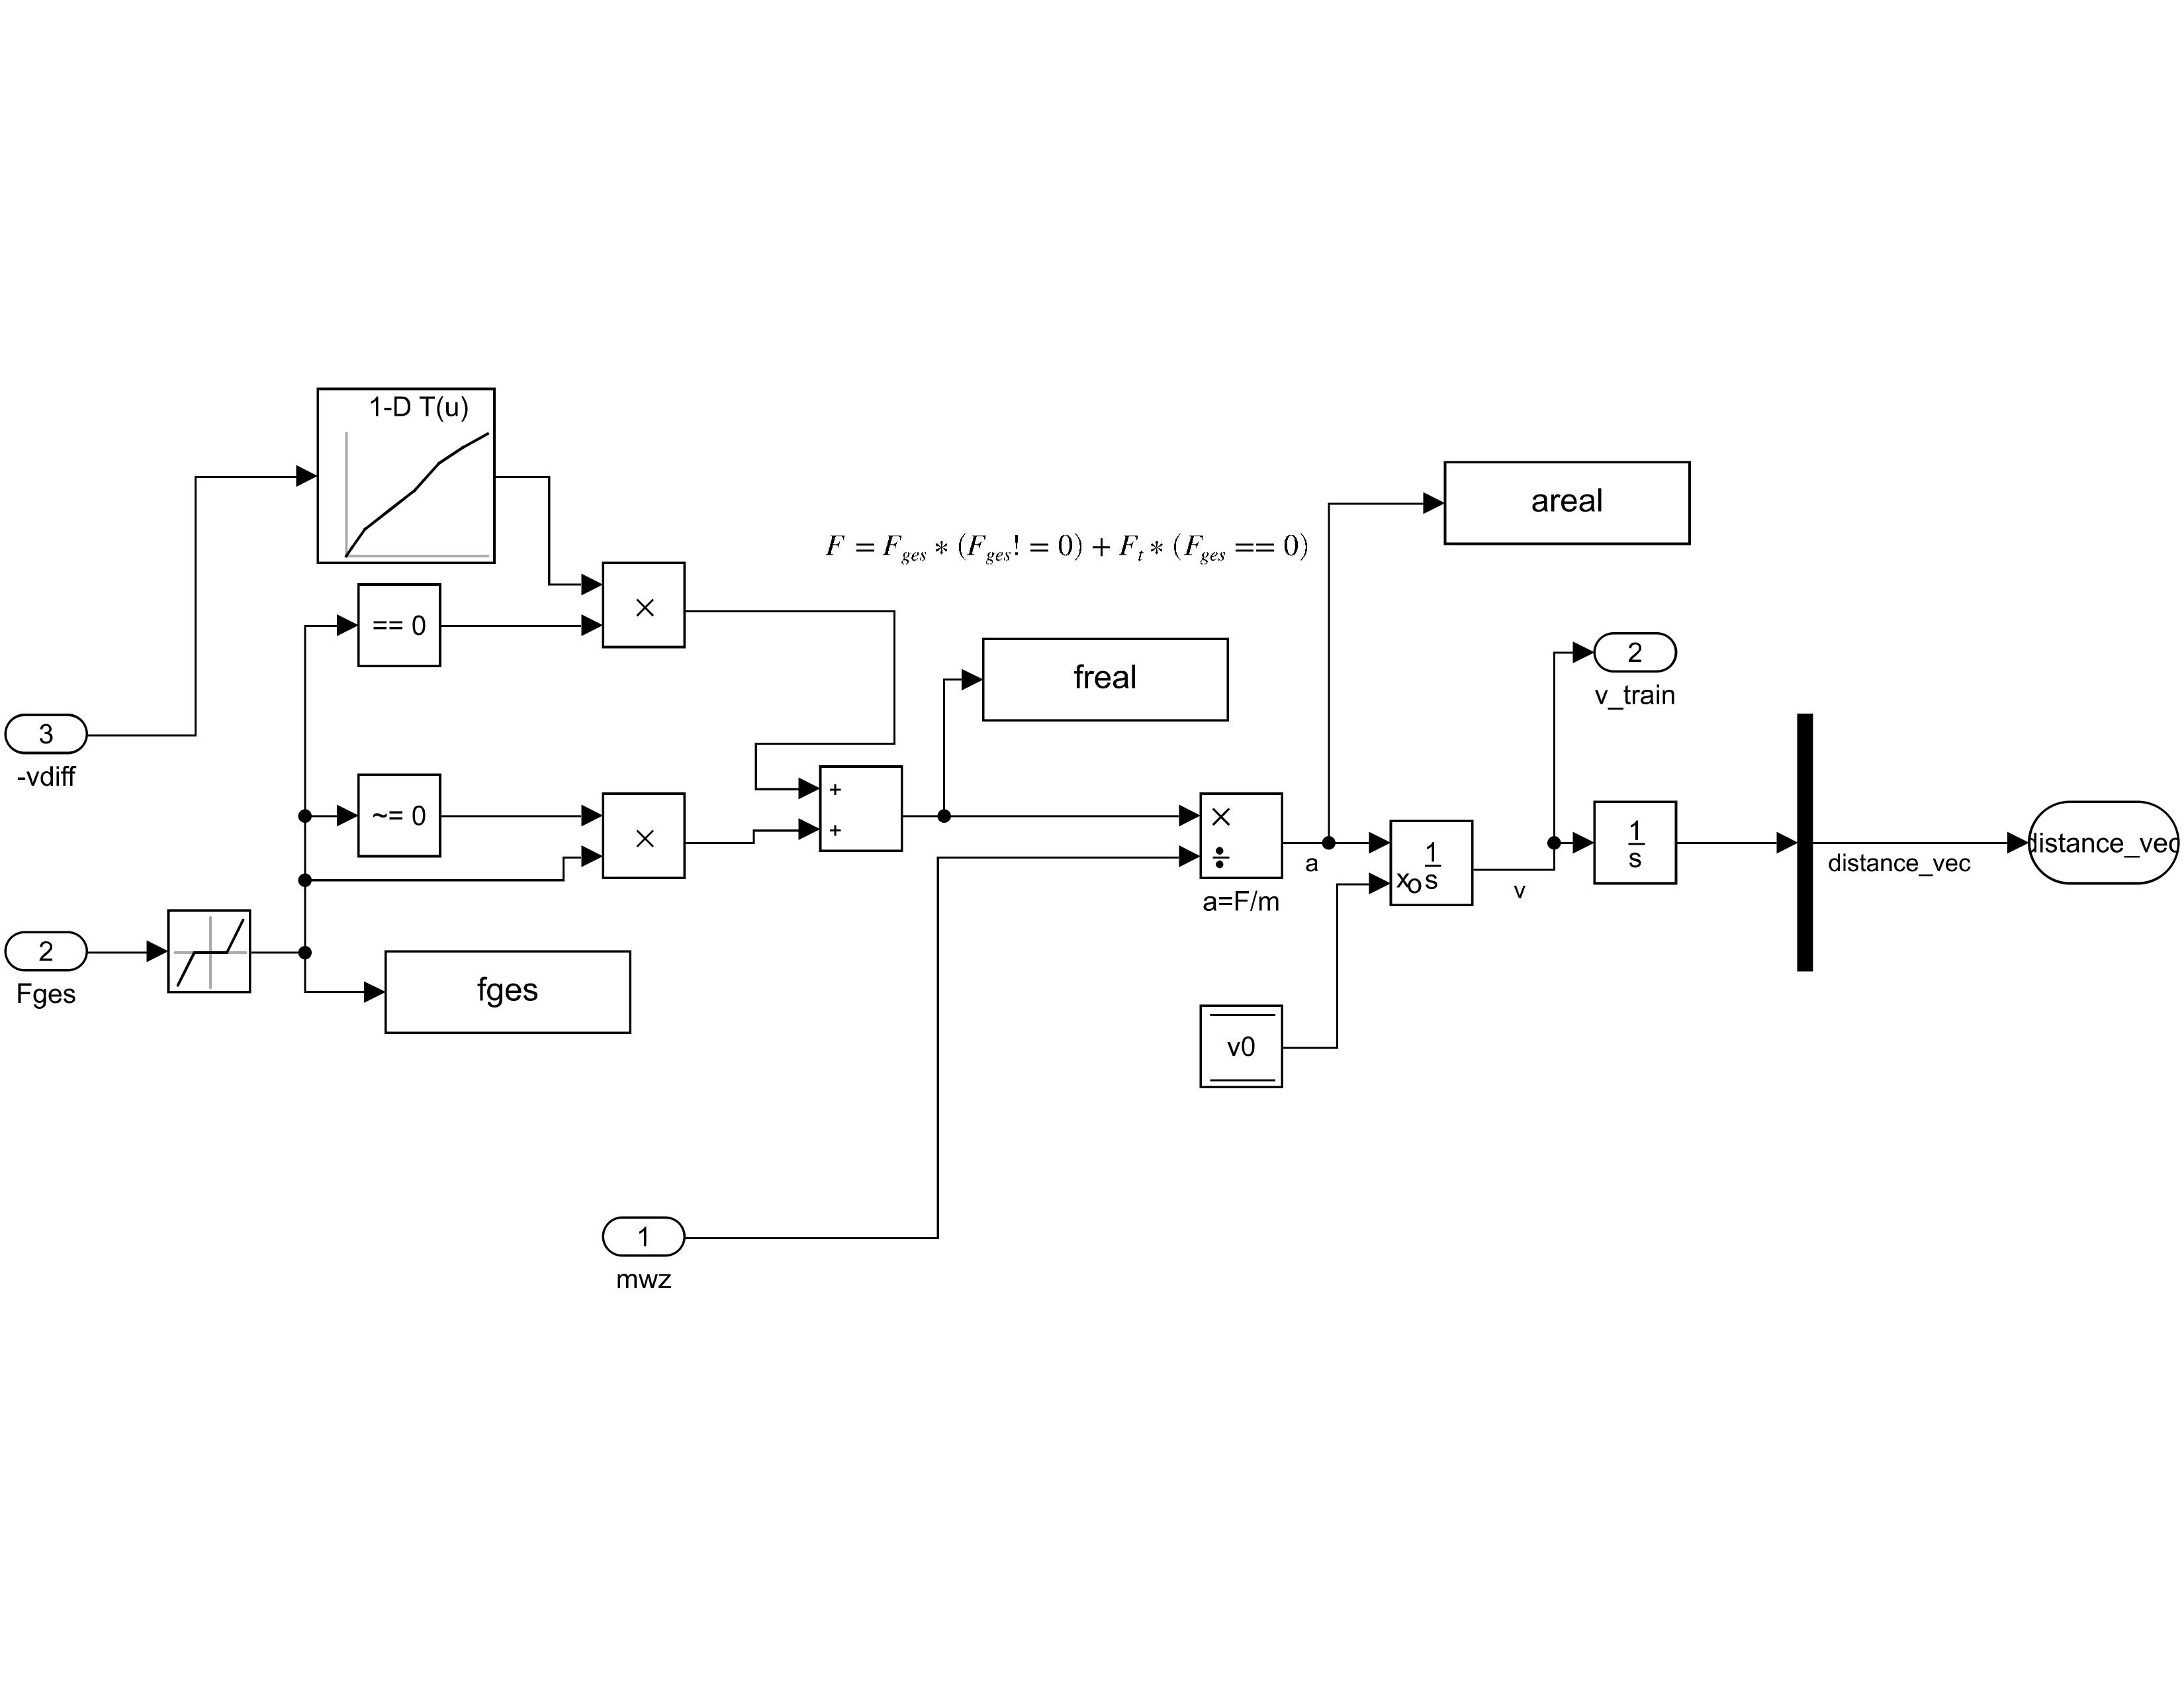
\includegraphics[width=\linewidth]{./pic/expandedmodel_force}
	\caption{Expanded Model - Traction Force Calculation}
	\label{fig:expandedmodel_force}
\end{figure}

\par\noindent
Figure \ref{fig:expandedmodel_force} shows the subsystem responsible for the calculation of the traction force, the train's acceleration, the train's velocity and the train's traveled distance. The applied traction force scales with $v_{dif}$ in a similar fashion to how $p_{bp}$ does. Again, a one-dimensional lookup table is used to calculate the appropriate value for $F_{t}$.

\begin{equation}
\label{eq:lookuptable2}
H(n) =
\begin{cases}
0.05 & \text{if $n=1$} \\
0.45 & \text{if $n=15$} \\
0.6 & \text{if $n=20$} \\
\text{..}
\end{cases}
\end{equation}

\noindent
Equation \ref{eq:lookuptable2} shows an example for how the function for the table might look like. The key difference to the calculation of the braking pressure is that the output values of the function are coefficients which are then multiplied with the maximum possible traction force, rather than raw values like in equation \ref{eq:lookuptable}. This part of the system is marked by the red rectangle. 
\par
Remember that we have established the train is at any given time either accelerating or decelerating. Since there is, as previously discussed, already a system in place to determine whether the train should engage its brakes, it now suffices to make the following examination: If the train is generating a braking force, i.e. $F_{b}$ is greater than zero, it will apply no traction force, and vice versa.
 
\begin{equation}
\label{eq:tracforce}
F_{t}(n,t) = (H(n) \cdot F_{t,max}) \cdot (F_{b}(n,t) == 0) 
\end{equation}

\noindent
Equation \ref{eq:tracforce} describes the logic. $F_{b}(t) == 0$ is a relational operation, the result being either 1 if there is a braking force at a particular point in time $t$, otherwise 0. We can apply the same logic to the braking force $F_{b}$:

\begin{equation}
\label{eq:brakeforce}
F_{b}(n,t) = F_{B}(n,t) \cdot (F_{b}(n,t) \neq 0)
\end{equation}

\noindent
With equations \ref{eq:tracforce} and \ref{eq:brakeforce} we can now determine the actual force applied at any given point in time $t$:

\begin{equation}
\label{eq:force}
F(n,t) = F_{t}(n,t) + F_{b}(n,t) 
\end{equation} 

\noindent
Since either of the summands is always zero, equation \ref{eq:force} outputs either the traction force or the braking force being applied at a point in time $t$, for a value of $v_{dif}$ $n$. This part of the system is marked by the blue rectangle, and together with the brake valve completes the system responsible for controlling the train.
\par\noindent
Let's reach back to our model ${\mathcal{M}}$ from chapter \ref{chap:FundamentalsOfRailwayVehicleEngineering}, in particular to three elements of its set of model variables $\{{\mathcal{V}}\}$: The train's acceleration $a$, its velocity $v$, and its braking distance $d$. Since we can now determine the applied force $F(n,t)$, it is now also possible to calculate the values of these three variables.

\begin{equation}
\label{eq:newton}
F = m \cdot a
\end{equation}

\noindent
Once again making use of Newton's second law of motion, we may calculate the value of $a$ by substituting $F(n,t)$ for $F$, and the combined mass of all wagons $m_{total}$ for $m$:

\begin{equation}
\label{eq:acceleration}
a = \frac{F(n,t)}{m_{total}}
\end{equation}
	
\noindent
The train's velocity may now be calculated by integration of its acceleration $a$. In simulink, this is achieved by feeding the signal value of $a$ into a continuous-time integration block:

\begin{equation}
\label{eq:velocity}
v = \int a \; da
\end{equation}

\noindent
Finally, the train's braking distance can be calculated by integration of its velocity $v$. This is once again achieved by usage of a continuous-time integration block:

\begin{equation}
\label{eq:distance}
d = \int v \; dv
\end{equation}

\noindent
This part of the system is marked by the green rectangle. This also completes the description of this subsystem. Looking back at our model ${\mathcal{M}}$, the last elements of $\{{\mathcal{V}}\}$ left to deal with are the brake pipe ${\mathcal{M}}_{bp}$, the brake cylinder ${\mathcal{M}}_{bc}$, the wagon mass $m$, the train composition $comp$, and finally the braking force $F_{b}$.

\begin{figure}[H]
	\centering
	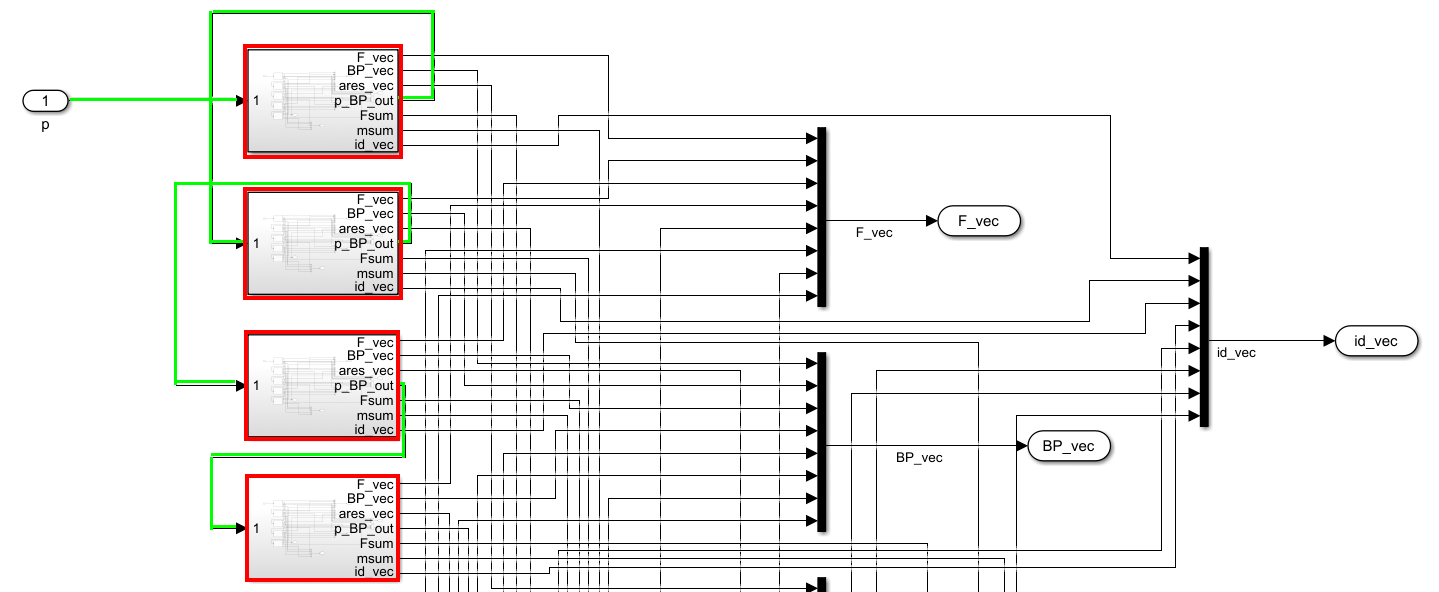
\includegraphics[width=\linewidth]{./pic/expandedmodel_brakepipe}
	\caption{Expanded Model - Brake Pipe}
	\label{fig:expandedmodel_brakepipe}
\end{figure}

\par\noindent
Figure \ref{fig:expandedmodel_brakepipe} shows how the wagons (marked by red rectangles) are interconnected by the brake pipe (marked by green arrows). This is analogous to how the wagons were connected in the initial model from section \ref{sec:InitialModel}.  

\begin{figure}[H]
	\centering
	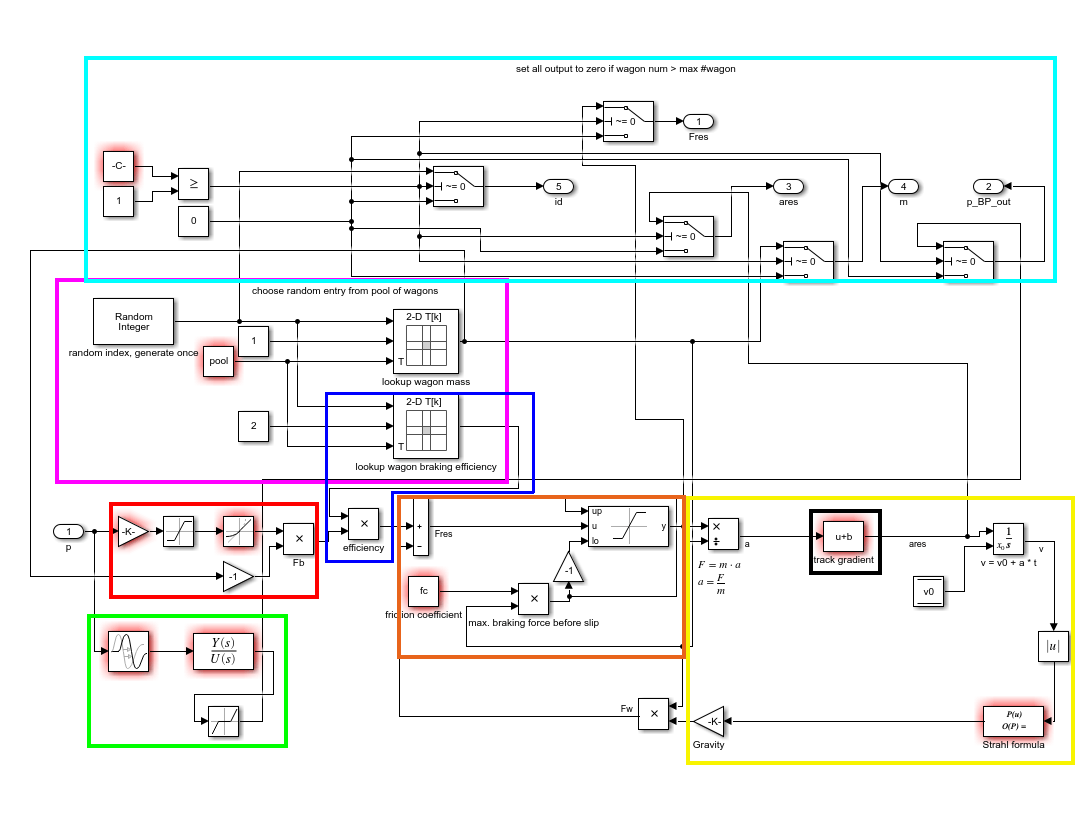
\includegraphics[width=\linewidth]{./pic/expandedmodel_wagon}
	\caption{Expanded Model - Wagon}
	\label{fig:expandedmodel_wagon}
\end{figure}

\par\noindent
Figure \ref{fig:expandedmodel_wagon} shows the expanded model of the freight wagon. There are components which have remained largely unchanged, while others have been added or altered to account for for the changes required to implement ${\mathcal{M}}$. To recapitulate, the initial model's freight wagon comprised of three components: The brake cylinder ${\mathcal{M}}_{bc}$, the brake pipe ${\mathcal{M}}_{bp}$, and the driving resistance. The implementation of the brake pipe has remained largely unchanged, the only exception being the addition of a dead zone to filter out very small values of $p_{bp}$, ranging from $-0.005$ to $0.005$. This was necessary as these small values interfered with the simulation result in a negative way. The implementation of the brake pipe ${\mathcal{M}}_{bp}$ is marked by the green rectangle.
\par
The implementation of the brake cylinder ${\mathcal{M}}_{bc}$ has also remained largely unchanged from the initial model, though the wagon's mass used to calculate $F_{b,max}$ is now read dynamically rather than being a static value (More on this later). The brake cylinder is marked by the red rectangle. The implementation of the calculation of the train's driving resistance has too remained unchanged except for the wagon's mass, used to determine the acceleration, being read dynamically, analogous to the brake cylinder. This component is marked by the yellow rectangle.
\bigskip
\par\noindent
According to the definition of ${\mathcal{M}}$, the following factors still need to be accounted for: The wagon mass $m$, the train composition $comp$, the track gradient $\alpha$, and the wheel/rail friction coefficient $\mu$. It is therefore necessary to add new components implementing these to the wagon model.
\par
While the initial model's wagons did indeed have a mass, it had a static value, and it was the same for all 40 wagons, making them identical and indistinguishable from one another. This is of course undesirable as it poorly reflects reality. To make up for this flaw, a pool of 500 wagons has been randomly generated via python script:

\bigskip
\begin{python}
import csv
import random

with open('pool.csv', 'w', newline='') as pool:
	fieldnames = ['Wagon_ID', 'Mass', 'Braking_eff']
	writer = csv.DictWriter(pool, fieldnames=fieldnames)
	
	writer.writeheader()
	for i in range(0,500): 
		mass = random.randrange(12000, 90000, 100)
		braking_eff = round(random.uniform(0.75, 0.95),2)
		writer.writerow({'Wagon_ID': i, 'Mass': mass, 'Braking_eff': braking_eff})
\end{python}
\bigskip

\noindent
This creates a table with 500 entries of the following structure:

\bigskip
\begin{table}[H]
	\label{tab:wagonpool}
	\centering
	\begin{tabular}{c|c|c}
		Wagon\_ID & Wagon Mass & Braking Efficiency \\
		\hline
		0 & 53800 & 0.83 \\
		\hline
		1 & 60800 & 0.77 \\
		\hline
		... & ... & ... \\
		\hline
		499 & 66600 & 0.81 \\
	\end{tabular}
	\caption{Wagon pool structure}
\end{table}

\bigskip

\noindent
Each wagon contained in the pool is identifiable by its ID and has the properties wagon mass and braking efficiency, i.e. a characteristic for the integrity of its brakes. Both properties are randomly generated for each wagon, the mass being assigned a value between 12000 and 90000 kilograms (with a step size of 100 kilograms), and the braking efficiency following a uniform distribution between 75 and 95 percent integrity. In order to read the values from the table, during simulation, each of the 40 wagon subsystems generates a random index between 0 and 499, i.e. each wagon is assigned an ID. By utilizing two direct lookup table blocks, the row with the assigned ID is selected, and the corresponding values for mass and braking efficiency are read from the table. The implementation of this component is marked by the pink rectangle. The value of $m$ is then used to calculate $F_{b}$, $a$, the driving resistance, the maximum braking force before slip, and the overall mass of the train $m_{total}$. The value of the braking efficiency is multiplied with $F_{b}$, meaning a lower integrity will result in a lower effective braking force. This component is marked by the blue polygon.
\par
The next element of ${\mathcal{V}}$ to address is the train composition $comp$. In the initial model, $comp$ is static, meaning the train is always comprised of 40 identical wagons. There is now a system in place that allows for wagons with diverse properties; we now need to design a system that allows for a variable number of wagons. In the simulink model, the train is made up of 40 subsystems, each representing one freight wagon. The obvious approach would be only having as many of these systems as desired, e.g. for a train consisting of 27 wagons, there would only be 27 wagon subsystems in the model. Since simulink however offers no straightforward way of adding or removing subsystems during simulation, a workaround is necessary. The solution taken here is using switch blocks to set output to zero for all unwanted subsystems, effectively removing their impact on the simulation. Each of the 40 models is assigned a constant representing their position; for each simulation, the desired number of wagons the train should encompass is specified as simulation input. During simulation, each subsystem compares this value to its position index. If their index is greater than the desired number of wagons, the switch blocks are set to output zero. For example, take a train of 15 wagons. The subsystems with position indices one to 15 will produce output, and the subsystems with indices 16 to 40 will not. This component is marked by the cyan rectangle.
\par
The track gradient $\alpha$ is used to calculate the additional braking or traction force resulting from the track's pitch angle. 

\begin{equation}
\label{eq:inclinationforce}
F_{N} = G_{F,Z} \cdot f_{N}
\end{equation}

\noindent
Equation \ref{eq:inclinationforce} is used to calculate the inclination force $F_{N}$, where $G_{F,Z} = m \cdot 9.81$ is the weight force acting on the wagon, and $f_{N} = \sin(\alpha)$ is the inclination force number [wende, 95]. Accordingly, this force is calculated during simulation and then added to (or subtracted from) the generated braking force $F_{b}$ to determine the effective braking force, taking into account the slope of the train track. This component is marked by the black rectangle.
\par
As mentioned in chapter \ref{chap:FundamentalsOfRailwayVehicleEngineering}, the wheel/rail friction coefficient $\mu$ determines how much braking force may be applied before sliding occurs, negatively impacting the braking performance. Since the exact mechanics of how sliding affects the braking process go beyond the scope of this work, a different approach has been chosen to incorporate $\mu$.

\begin{equation}
\label{eq:frictioncoefficient}
F_{b,e} = F_{b,max} \cdot \mu
\end{equation}

\noindent
Equation \ref{eq:frictioncoefficient} is used to calculate the braking force before sliding would occur, $F_{b,e}$ by multiplying the maximum possible braking force $F_{b,max}$ with the wheel/rail friction coefficient $\mu$. The result is then used to limit the applied braking force $F_{b}$ so that sliding is avoided, utilizing a saturation dynamic block. This still satisfies $R_{\mu,F_{b}} \in \{ {\mathcal{R}} \}$. This component is marked by the brown rectangle.
\bigskip
\par\noindent
This completes the description of the simulink model. Reaching back to chapter \ref{chap:FundamentalsOfRailwayVehicleEngineering}, all elements of $\{ {\mathcal{V}} \}$, $\{ {\mathcal{R}} \}$ and $\{ c \}$ have been accounted for, and we can therefore conclude our theoretical model ${\mathcal{M}}$ has been implemented. It may now be used for simulation and data generation.

\section{Outlook}
\label{sec:Outlook}

\par\noindent
While the model defined in chapter \ref{chap:FundamentalsOfRailwayVehicleEngineering} satisfies the requirements for this work, there are many more factors that might be incorporated in order to achieve a more accurate representation of reality. Some of these factors shall be discussed here briefly. So far, the generated braking force $F_{b}$ is calculated by transforming the braking pressure $p_{bp}$ into a coefficient, and applying that coefficient to the maximum braking capacity $F_{b,max}$.

\begin{equation}
\label{eq:brakingforceadjusted}
F_{b} = \xi \cdot \sum P_{N}
\end{equation}

\noindent
Equation \ref{eq:brakingforceadjusted} offers a more detailed way of calculating $F_{b}$, where $\sum P_{N}$ is the sum of all applying forces actuating the brake shoes on the wheel tread, or the brake pads against the discs, respectively; the proportionality coefficient $\xi$ might be the friction coefficient between the brake shoes and the wheel, or

\begin{equation}
\label{eq:xi}
\xi = \frac{4 \cdot r_{m}}{D_{o}} \cdot \mu_{d}
\end{equation}

\noindent
for disc brakes, where $r_{m}$ is the medium friction radius, $D_{o}$ is the wheel diameter, and $\mu_{d}$ is the friction coefficient between brake pad and disk [train braking, 23].
\par
As the focus of this work lies on the braking process, the modeling of traction force is kept rather simple. It might however be desirable to create a more sophisticated model, in order to achieve a more realistic result. For example, as of right now, the applied traction force depends only on the discrepancy between current and maximum velocity; in reality, the maximum traction force is also limited by wheel/rail adhesion just as the braking force is [wende, 157]. One might also want to factor in differences between various engines.
\chapter{Data Generation}
\label{chap:DataGeneration}
\par\noindent
\textit{\textbf{Introduction}} With the finished model, it is now possible to generate the actual data, via simulation. For this purpose, a matlab script initializes all relevant model parameters and feeds the simulation input, in this case the previously discussed track profile, into the model. 

\begin{figure}[H]
	\centering
	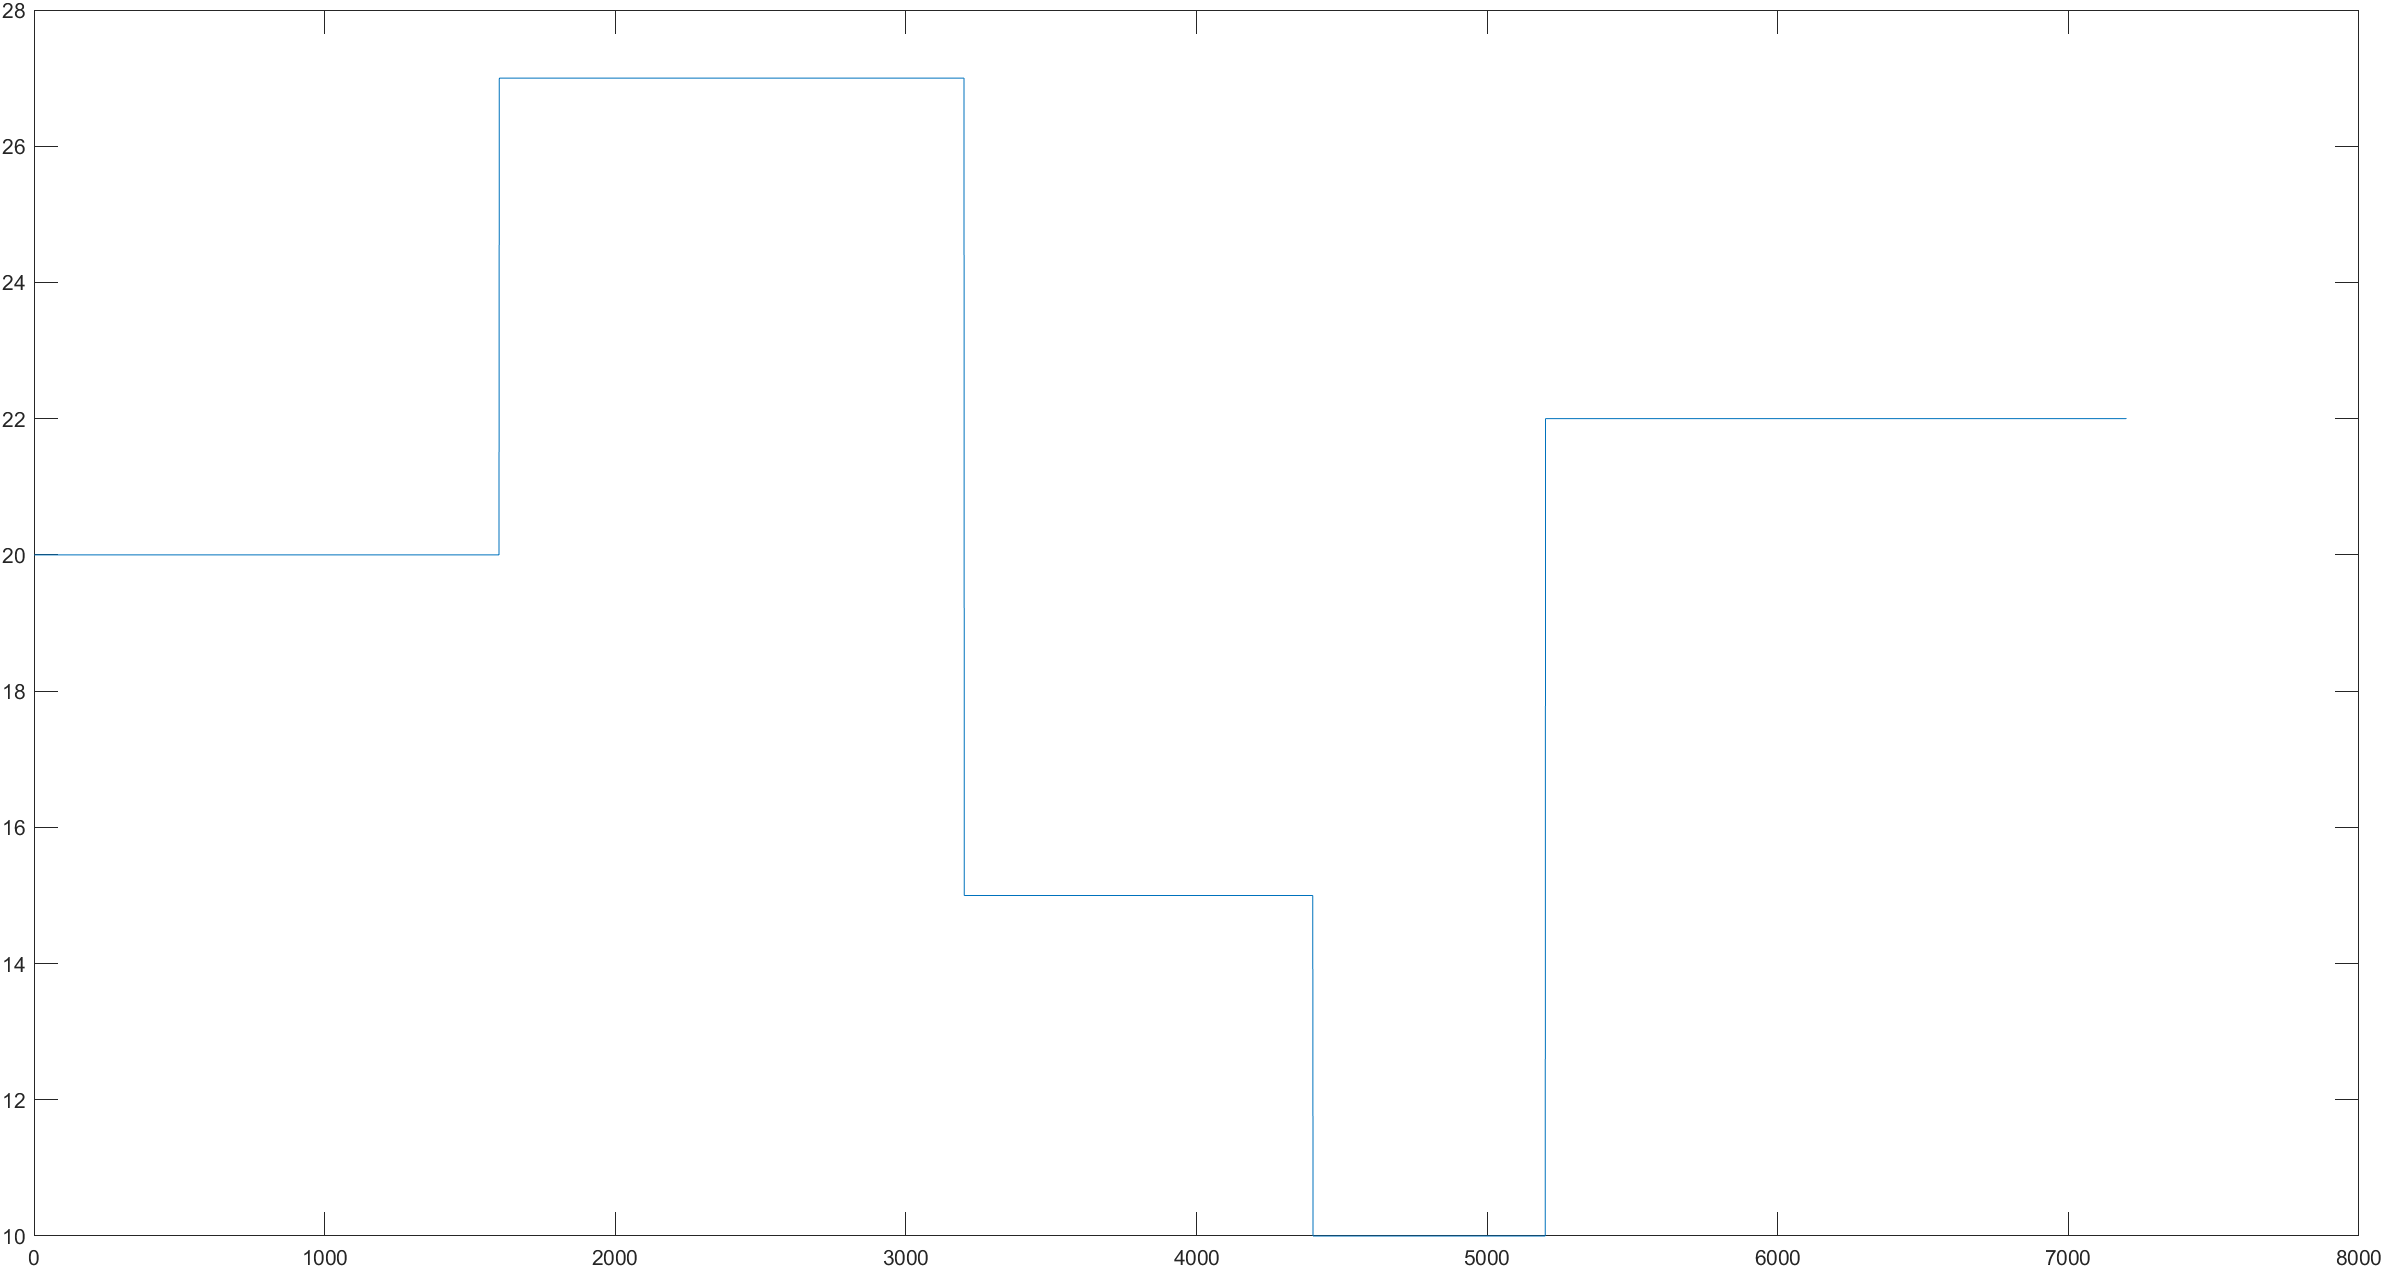
\includegraphics[width=\linewidth]{./pic/input}
	\caption{Simulation Input}
	\label{fig:siminput}
\end{figure}

\par\noindent
Figure \ref{fig:siminput} visualizes how a track profile might look like. It stipulates the maximum allowed velocity for discrete points in time; the train either brakes or accelerates accordingly in order to match the corresponding value. An example: Let the simulation time be 1200 seconds, and $v_{max}(1200)=20 \; \frac{m}{s}$. Let the train's velocity $v$ be $25 \; \frac{m}{s}$. The train will engage its brakes (or continue braking, if they have already been engaged) in order to bring $v$ down to $20 \; \frac{m}{s}$. If $v$ were $15 \; \frac{m}{s}$, the train would accelerate instead.

\section{Matlab Code}
\label{sec:MatlabCode}
\par\noindent
We need to do some general configuration first, like clearing the workspace off all output which might still be present from previous simulations. 

\begin{lstlisting}
%% Initialise
clear all
clc
warning ('off','all');
numcores = 10; % configure number of cores to use in parallel processing
\end{lstlisting}

\par\noindent
We then need to initialise all constants which values remain the same for all simulations. Please refer to the code snippet below for descpriptions:

\begin{lstlisting}
%% Constants

RBD = 5; % regular operations pressure (bar)
VBD = 3.5; % full breaking pressure (bar)

l = 18; % wagon length (meters)
c = 250; % propagation velocity (km/h)

tf = 4; % brake cylinder filling time
tl = .1; 

p0 = 0; % initial pressure
Pres = 0/1000*[5.7/771 0 1.6]; % strahl formula for m/s velocity

alpha = 0.9; 

BPnum = [0.3 alpha]; 
BPden = [1 alpha]; 

%% Simulation input
tmax = 3600; % simulation time (seconds)
nmax = tmax * 2; % number of data points
t = linspace(0, tmax, nmax); % simulation time input
u = [20*ones(800*2,1); 27*ones(800*2,1); 15*ones(600*2,1); 10*ones(400*2,1); 
	22*ones(900*2,1); 0*ones(100*2,1)]; % track profile
simin.time = t; % set simulation time input
simin.signals.values = u; % set simulation signal input

trackgradient = 0; % pitch angle
\end{lstlisting}

\par\noindent
After having initialised all necessary constants, we now get to configuring variable simulation input.

\begin{lstlisting}
pool = readmatrix('pool.csv'); % read wagon pool
mkdir output; % make output directory

wagons = 1:1:40; % create array for number of wagons to loop over
friction = 0.05:0.01:0.78; % create array for friction coefficient to loop over
tracforce = 200000:1000:400000; % create array for traction force to loop over

track = 1; % counter to index input array for one batch of simulations
allruns = 1; % counter to keep track of total number of simulations completed

for i = length(tracforce):-1:1 		% all possible combinations of traction force,
	for j = length(friction):-1:1 	% friction coefficient and
		for k = length(wagons):-1:1 % number of wagons
			% save all previously initialised constans and sim input into
			% one array in
			in(track) = Simulink.SimulationInput('Simulation_v2');
			in(track) = in(track).setVariable('num_wagons',wagons(k));
			in(track) = in(track).setVariable('fc',friction(j));
			in(track) = in(track).setVariable('Ft',tracforce(i));
			
			in(track) = in(track).setVariable('alpha',alpha);
			in(track) = in(track).setVariable('BPden',BPden);
			in(track) = in(track).setVariable('BPnum',BPnum);
			in(track) = in(track).setVariable('c',c);
			in(track) = in(track).setVariable('l',l);
			in(track) = in(track).setVariable('nmax',nmax);
			in(track) = in(track).setVariable('p0',p0);
			in(track) = in(track).setVariable('pool',pool);
			in(track) = in(track).setVariable('Pres',Pres);
			in(track) = in(track).setVariable('RBD',RBD);
			in(track) = in(track).setVariable('simin',simin);
			in(track) = in(track).setVariable('t',t);
			in(track) = in(track).setVariable('tf',tf);
			in(track) = in(track).setVariable('tl',tl);
			in(track) = in(track).setVariable('tmax',tmax);
			in(track) = in(track).setVariable('trackgradient',trackgradient);
			in(track) = in(track).setVariable('u',u);
			in(track) = in(track).setVariable('VBD',VBD);
			
			% also save the respective values for traction force and
			% friction coefficient into arrays
			Ft(track) = tracforce(i);
			fc(track) = friction(j);
			
			track = track + 1;       
		end
	end
	
	fprintf('Starting pool for %d simulation runs.\n',length(in));
	parpool(numcores); % create a pool of #numcores workers for parallel processing
	out = parsim(in,'ShowProgress','on'); 	
	% start parallel simulations for all
	% entries of in, save output to out
											
	matrix = []; % create an empty matrix
	
	parfor l = 1:1:length(out) 	
	% parallel loop over out, which is an array that
	% holds all simulation outputs
	
		tmp = Write(l + allruns,out(l).get('velocity'),out(l).get('force')
			,out(l).get('pressure'),out(l).get('distance'),
			out(l).get('acceleration_neg'),out(l).get('ids'),t,u,
			trackgradient,Ft(l),fc(l)); % for each entry, pack all output into one single matrix
		matrix = [matrix;tmp]; % append to matrix
	end
	
	allruns = allruns + length(out); % update total number of simulations

	writematrix(matrix,'output/output.tsv','FileType','text','WriteMode','append',
		'Delimiter','tab'); 
	% write matrix, which holds all output matrices of the 
	% current batch, to a tsv file

	track = 1; % reset batch index 
	delete(gcp('nocreate')); % delete parallel pool
	fprintf('Run %d (of %d total) complete.\n',length(tracforce)-i,length(tracforce));
end
\end{lstlisting}

\par\noindent
As our aim is to generate large quantities of data, it becomes feasible to use use parallel processing for our simulations. For this purpose, we need to create an array to hold input for all simulation runs. There are three variables which change for each run, they are traction force of the locomotive, wheel/rail friction coefficient and number of wagons, respectively. A nested loop is used to create all possible combinations of these variables, and each single combination gets stored, as a new entry, in the array which holds all input.
\par
Variable ranges are from one to 40 for number of wagons, .05 to .78 for friction coefficient and 200000 to 400000 for traction force, with step sizes one, .01 and 1000 respectively. We therefore have a total number of $40*74*200 =  592000$ combinations. The obvious approach here would be to generate the full batch of 592000 input configurations, but performance and hardware limitations proved this to be unfeasible. Instead, we use rather small batche sizes of 2960 for parallel simulation.
\par
Writing of the output is also done in smaller batches. The best approach to minimize the number of file accessions is of course writing everything into one big matrix, thus storing in RAM, and then writing the matrix in one go. Unfortunately, growing an array by assignment or concatenation can be expensive. For large arrays, MATLAB must allocate a new block of memory and copy the older array contents to the new array as it makes each assignment. The other extreme would of course be to write every single output line directly, but the large number of file accessions required makes this even more unfeasible, so a middle ground is needed, and a batch size of ~3000 works relatively well, although this could surely be optimized with a bit of runtime analysis.
\par
The function below compresses all output of one single simulation into one matrix. Raw simulation output consists of a few time-series objects, like braking force and braking pressure, as well as some metadata. These objects are fed into the write function, which does as many loops as there are rows in the time-series objects. It then packs all rows from each time-series into one big row, adds the meta-data and appends the large row to the matrix, which gets returned at the end. Refer to section \ref{sec:DataStructure} for a more detailed look at the structure of the output matrix.

\begin{lstlisting}
function ret = Write(id,velocity,force,pressure,distance,acceleration,wagon_ids,t,u,grad,ft,fc)
	numrows = get(force,'Length');
	wagon_ids = double(wagon_ids);
	time = force.Time;
	matrix = [];
	
	for i = 1:1:numrows
		f = getdatasamples(force,i);
		p = getdatasamples(pressure,i);
		v = getdatasamples(velocity,i);
		a = getdatasamples(acceleration,i);
		d = getdatasamples(distance,i);
		
		row = [id,time(i),f,p,v,a,d,wagon_ids,grad,ft,fc]; 	% TODO: add simulation input aka track profile to matrix
		%		print wagon ids as list delimited by colon (,)
		%		performance?
		matrix = [matrix;row];
	end
	fprintf('Created output matrix for simid %d\n',id);
	% writematrix(matrix,'output/output.tsv','FileType','text','WriteMode','append','Delimiter','tab');
	% ret = 1;
	% fprintf('Create output matrix for Simulation ID %d\n', id);
	ret = matrix;
end
\end{lstlisting}

\begin{lstlisting}[language=python]
import csv
import random

with open('pool.csv', 'w', newline='') as pool:
	fieldnames = ['Wagon_ID', 'Mass', 'Braking_eff']
	writer = csv.DictWriter(pool, fieldnames=fieldnames)
	
	writer.writeheader()
	for i in range(0,500): # create 500 randomized wagons
		mass = random.randrange(12000, 90000, 100) # create random wagon mass between 12 t and 90 t with step size 100
		braking_eff = round(random.uniform(0.75, 0.95),2) # create random braking efficiency as uniform distribution between 75 % and 95 %
		writer.writerow({'Wagon_ID': i, 'Mass': mass, 'Braking_eff': braking_eff})
\end{lstlisting}

\par\noindent
The above python script is used to create a randomized pool of 500 wagons to be used in simulation. Each wagon has a unique id, a randomized mass, ranging between 12000 and 90000 kilograms, and a braking efficiency, which is a uniform distribution between .75 and .95.

\section{Data Structure}
\label{sec:DataStructure}
\par\noindent
As has been denoted previously, generated data should be suitable for big data processing. The first approach was to create a new directory for each iteration, and also save the different parameters to different files. Since this is very inefficient in terms of number of file accessions and therefore negatively impacts performance, as well as being unsuitable for transformations to big data file systems like Apache Hadoop or Apache Hive, it has been proposed to write all output into one single file. Let's take a look at the structure first.

\begin{tabular}{|c|c|c|c|c|c|c|c|c|c|c|c|c|c|c|c|c|}
	\hline
	simID & Timestamp & $F_{wagon0}$ & ... & $P_{wagon0}$ & ... & $v_{wagon0}$ & ... & $a_{wagon0}$ & ... & Distance & Wagons & Track angle (tentative) & $F_{t}$ & fc & Track profile \\
	\hline
	&  &  &  &  &  &  &  &  &  &  &  &  &  &  &  &  \\
	\hline
	&  &  &  &  &  &  &  &  &  &  &  &  &  &  &  &  \\
	\hline
	&  &  &  &  &  &  &  &  &  &  &  &  &  &  &  &  \\
	\hline
	&  &  &  &  &  &  &  &  &  &  &  &  &  &  &  &  \\
	\hline
	&  &  &  &  &  &  &  &  &  &  &  &  &  &  &  &  \\
	\hline
	&  &  &  &  &  &  &  &  &  &  &  &  &  &  &  &  \\
	\hline
\end{tabular}

\par\noindent
Some output objects are time-series, namely braking force, braking pressure, acceleration, distance and velocity. Force, pressure and acceleration, which get measured for every wagon, look like this

\begin{tabular}{|c|c|c|c|c|}
	\hline
	Timestamp & $Wagon_{1}$ & $Wagon_{2}$ & ... & $Wagon_{40}$ \\
	\hline
	0 & 0 & 0 & 0 & 0 \\
	\hline
	10 & $x_{1}$ & $x_{2}$ & ... & $x_{40}$ \\
	\hline
	... & ... & ... & ... & ... \\
	\hline
	3600 & $y_{1}$ & $y_{2}$ & ... & $y_{40}$ \\
	\hline
\end{tabular}

\par\noindent
whereas distance and velocity only have two columns and thus look like this

\begin{tabular}{|c|c|}
	\hline
	Timestamp & Value \\
	\hline
	0 & 0 \\
	\hline
	.. & .. \\
	\hline
	3600 & $x$ \\
	\hline
\end{tabular}

\par\noindent
Since they all posses the same number of lines, which is the number of timestamps at which measurements were taken, all columns from all these objects may be compressed into a single table. All columns containing meta-information, for example simulation id, which theoretically only needs to be printed once, get filled with the same value for all lines, and since the number of wagons may vary from one to 40, all possibly empty columns get filled with zeros, so that we do not get any columns containing no value. 

\section{Analysis of generated Data}
\label{sec:AnalysisOfGeneratedData}
\chapter{Performance Analysis}
\label{chap:PerformanceAnalysis}
\section{Conclusion}
\label{sec:Conclusion}


% Nachspann
\nocite{Segmentation} % Quelle wird nicht im Text erwähnt -> Quellenverzeichnis
\nocite{ImageAttack}
% Weitere quellen müssen in 'bib/quellen.bib' eingetragen werden
% !!! -> BibTex ausführen! Sonst tauchen die Quellen nicht im Verzeichnis auf.

% Quellenverzeichnis
\clearpage
%\bibliographystyle{alpha}
%\bibliographystyle{apalike}
%\bibliography{./bib/quellen}
%\addcontentsline{toc}{chapter}{Quellenverzeichnis}
%\addtocontents{toc}{\vspace{0.8cm}}

% Abkürzungsverzeichnis
%\clearpage
%\markright{Abkürzungsverzeichnis}
%\include{./doc/202abkuerzungsverzeichnis}
%\addtocontents{toc}{\vspace{0.8cm}}

% Abbildungsverzeichnis
\clearpage
\addcontentsline{toc}{chapter}{Abbildungsverzeichnis}
\listoffigures
\addtocontents{toc}{\vspace{0.8cm}}

% Tabellenverzeichnis
\clearpage
\addcontentsline{toc}{chapter}{Tabellenverzeichnis}
\listoftables
\addtocontents{toc}{\vspace{0.8cm}}

% Anhaenge
\addcontentsline{toc}{chapter}{Anhang}
\appendix
%\input{./app/Dateiname}
\chapter{Quellcode}
\begin{enumerate}
      \item Source 1
      \item Source 2
\end{enumerate}

% Anhänge im Ordner 'app' ablegen

%\includepdf[pages=1-4]{./app/Datenblatt1.pdf} % Datei mit 4 Seiten
%\includepdf[pages=1]{./app/Datenblatt2.pdf} % Datei mit einer Seite

\chapter{Data visualization}

%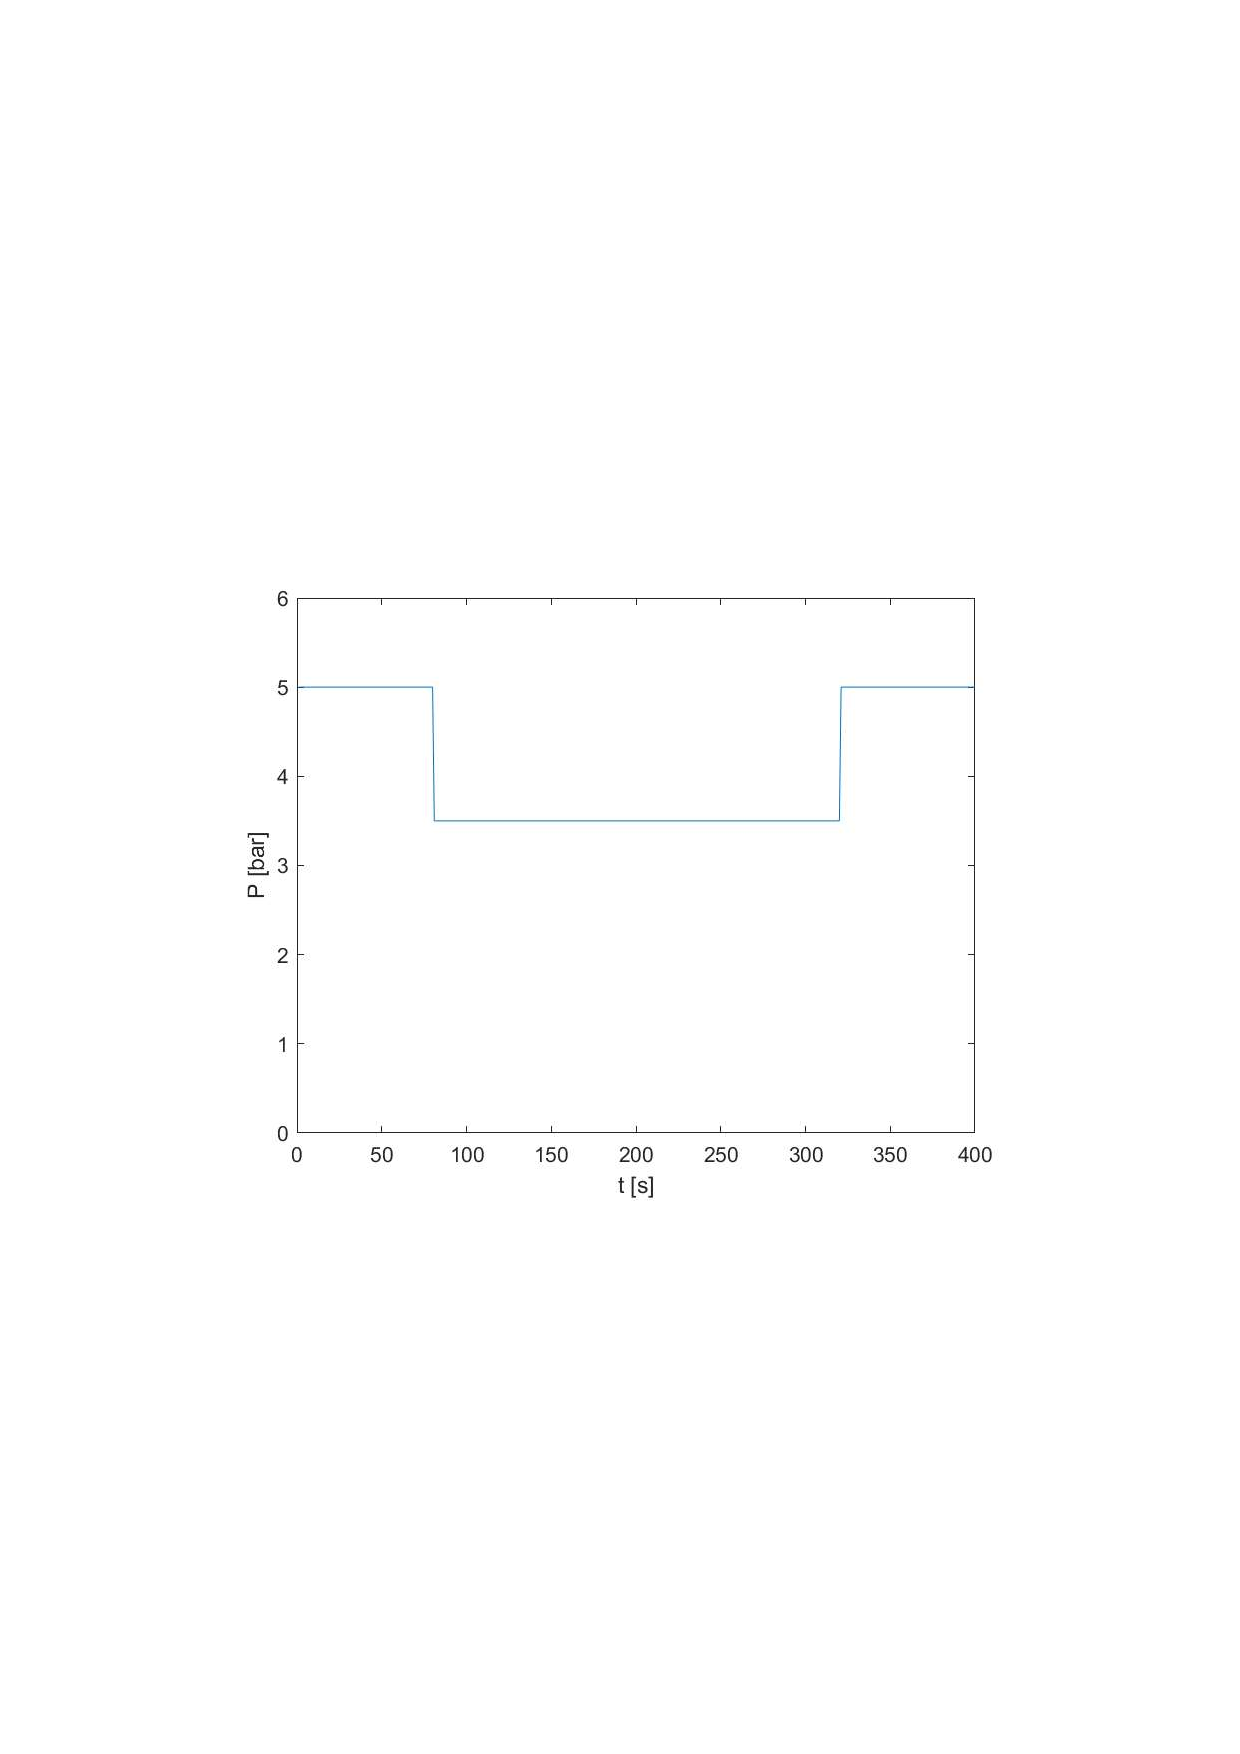
\includepdf{./app/initmodel_pressureinput.pdf}
\TODO{Visualisierungen einfügen}
\begin{center}
	Initial model - simulation input
	\label{fig:initmodel_siminput}
	Expanded model - simulation input
	\label{fig:expandedmodel_siminput}
\end{center}



\end{document}
